\chapter{Separation by Unknown Modulation}
\label{cha:unknown}

In the previous chapter, methods were proposed to separate highly overlapped signals, informed by an estimate of pitch variation of the source to be separated.
Even though, I showed that pitch variation can be estimated from the mixture, often, it is not easy to obtain in practice.
In contrast, in this chapter, I will introduce separation methods which do not incorporate prior knowledge about the modulation. 
In fact, some of the methods operate blindly, meaning they do not require any further information about the sources except for the number of sources to be separated.
\par
% \section{Modulation Spectrogram based Separation}
% Intro commonfate START
% Unknown modulation!
In blind source separation research, many contributions in the past were based on non-negative matrix factorization (NMF)~\cite{lee99, lee01}.

NMF quickly became one of the main scientific frameworks in the field of audio source separation with a large number of contributions.
The popularity of NMF algorithms can be explained by the intuitive way in which they work on (non-negative) time-frequency representations of the mixture signal.
Assuming the magnitude STFT \(\mX \in \sR_{+}^{F \times T}\), NMF incorporates non-negative constraints to perform the separation into the sum of \(K\) components which are each factored into two matrices (usually referred to as \emph{basis} \(\mW_{+} \in \sR^ { F \times K }\) and \emph{activations} \(\mH_{+} \in \sR^ { T \times K }\)). 

\begin{equation}
   \mathbf{V} \approx \mW \mH^{T} = \sum\limits_{j=1}^{K} \vw_{j} \circ \vh_{j} 
   \label{eq:vanilla_nmf}
\end{equation}

As it can be seen, the NMF product can also be written as the outer product between two rank-1 matrices (using the \(\circ\)-operator); this is visualized in Figure~\ref{fig:nmf}.

\begin{figure}[h]
  \centering
  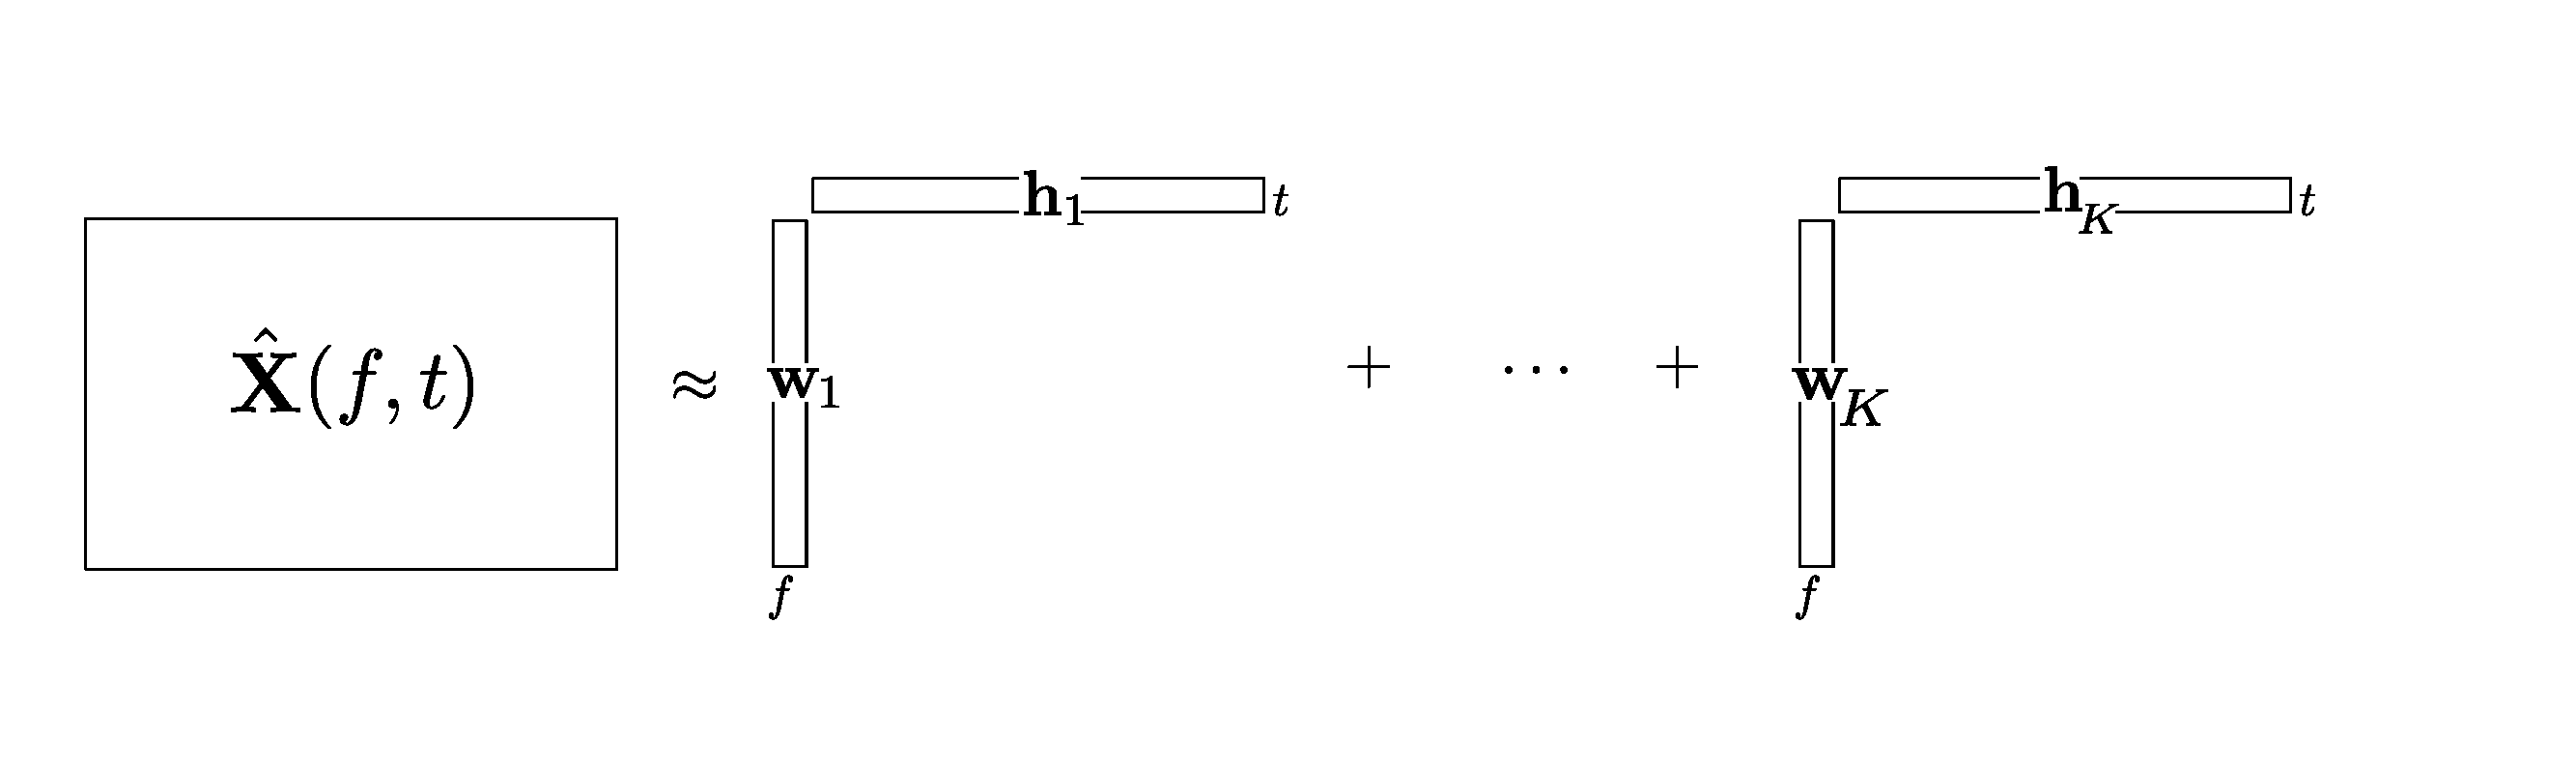
\includegraphics[width=0.8\textwidth]{Chapters/06_Separation_Unknown/figures/nmf.pdf}
  \caption{Non-negative matrix factorization}
  \label{fig:nmf}
\end{figure}

The NMF provides a rank reduction which is needed to decompose mixtures into (\(K\)) source components.
At the same time, the factorization inherently follow specific properties of music spectrograms which is the fact that harmonic sources have be described using a pitch/tone based dictionary (\(\mW\)) and its note activations (\(\mH\)).
In Figure~\ref{fig:nmf_separation}, an example where this is demonstrated in a simple example, is depicted.

\begin{figure}
  \centering
  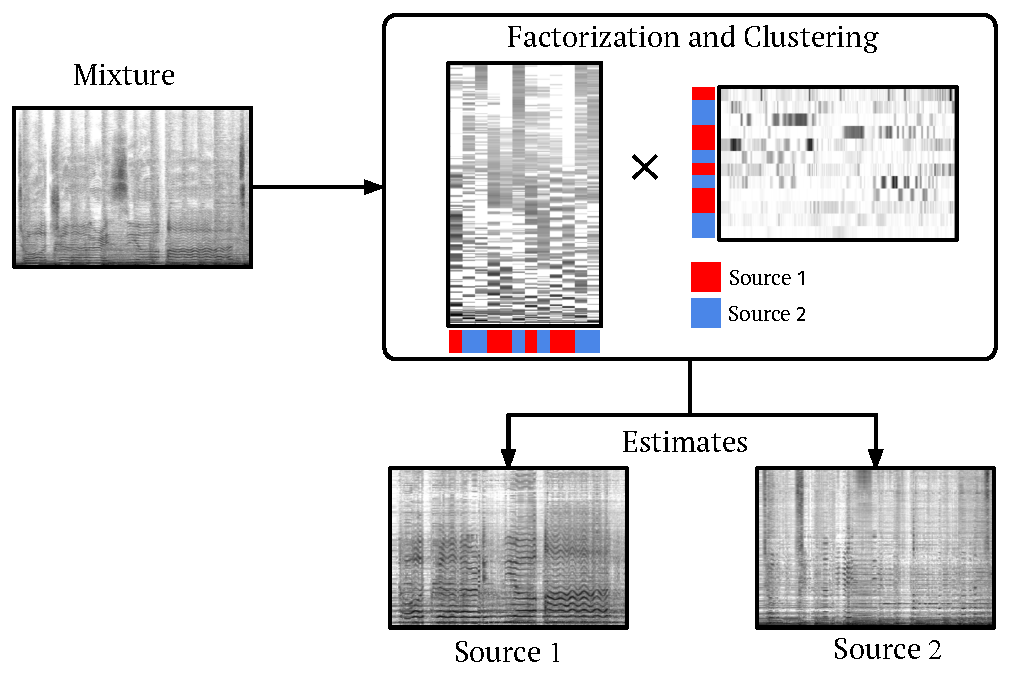
\includegraphics[width=0.8\textwidth]{Chapters/06_Separation_Unknown/figures/nmf_separation.pdf}
  \caption{NMF}
  \label{fig:nmf_separation}
\end{figure}

It is this property that also allowed to use NMF for the purpose of transcriptions~\cite{smaragdis03}.
\par
% stolen from somewhere
After factorizing into its \(K\) components, one can easily obtain \(K\) magnitude spectra.
However, \(K\) is usually selected to be larger or equal to the total number of sources.
When it is larger than the number of sources, components can be clustered into the number of desired sources.
Often this can be achieved by some similarity metric that compares the \(k\)-th component with one of the desired sources by a \textit{k}-means clustering algorithm~\cite{spiertz09}.
It is exactly this step that transforms the NMF as an unsupervised algorithm into a supervised algorithm.
As for other spectrogram based methods, separation is performed using Wiener filters to extract the sources from the mixture~\cite{liutkus15c}.
\par

% from zafar...
The first work on NMF based audio separation was proposed by Vembu and Baumann in~\cite{vembu05}. 
They used NMF to separate vocals from mixtures and first discriminated between vocal and non-vocal sections in a mixture by using different combinations of features, such as MFCCs \cite{david80}. The components were then grouped as vocal and non-vocal by reusing a vocal/non-vocal classifier with MFCC coefficients.
% end zafar...
Since then a la large variety NMF ``flavors'' were introduced to deal with certain aspects of the NMF for the application of Music. 
Many of then can be found in Chapter 16 of~\cite{vincent}.
Here the authors also describe one of the main problems with NMF which is that ``standard NMF is shown to be efficient when the notes of the analyzed music signal are nearly stationary''.
As I showed in Chapter~\ref{cha:highly-overlapped-signals}, this is especially false for notes that incorporate vibrato.
This becomes a problem for NMF based processing because with a representation based on a standard NMF and the magnitude spectrogram, it is hard to model these sources with only a few spectral templates. 
\par
To underpin this issue, I depict this problem in Figure~\ref{fig:am_tensor}, where I show the factorization of a simple amplitude modulated input signal for comparison. 
The signal consists of two sinusoids which are linearly mixed. 
Both share the same carrier frequency but have different amplitude modulation frequencies. 
I choose a factorization into $K=2$ components. 
From the activation components one can see that NMF is not able to separate the two signals sufficiently. 
% TODO
\begin{figure}[h]
\centering
\subcaptionbox{Time Domain}%
[1\textwidth]{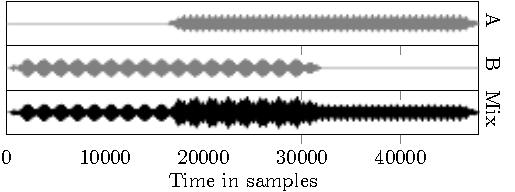
\includegraphics[width=0.8\textwidth]{Chapters/05_Separation_Known/figures/Timepdf-crop.pdf}}%
\hspace{0.2\textwidth} % separation
\subcaptionbox{Magnitude STFT}
[1\textwidth]{% This file was created by matlab2tikz% This file was created by matlab2tikz v0.4.7 (commit 3442858e5a642c135c5e9dab6a960bee5b9c6f8d) running on MATLAB 8.2.
% Copyright (c) 2008--2014, Nico Schlmer <nico.schloemer@gmail.com>
% All rights reserved.
% Minimal pgfplots version: 1.3
%
% The latest updates can be retrieved from
%   http://www.mathworks.com/matlabcentral/fileexchange/22022-matlab2tikz
% where you can also make suggestions and rate matlab2tikz.
%
\begin{tikzpicture}[font=\small]

\begin{axis}[%
width=0.225\columnwidth,
height=3.5cm,
axis on top,
xminorgrids=true,
minor xtick={1.5,2.5},
scale only axis,
xtick={1,2},
xmin=0.5,
xmax=2.5,
ymin=0.5,
ymax=137.5,
name=plot2,
xlabel=Gain Components,
ylabel=Modulation Frequency Bins,
every axis y label/.style={at={(current axis.north east)},below=18mm,xshift=4mm},
y label style={rotate=-90},
]
\addplot [forget plot] graphics [xmin=0.5,xmax=2.5,ymin=0.5,ymax=137.5] {Chapters/dafx/figures/AMPlots/GAS-1_scaled.png};
\end{axis}

\begin{axis}[%
width=0.225\columnwidth,
height=3.5cm,
xminorgrids=true,
minor xtick={1.5,2.5},
axis on top,
scale only axis,
xtick={1,2},
xmin=0.5,
xmax=2.5,
ymin=0.5,
ymax=145.5,
xlabel=Basis Components,
ylabel=Frequency Bins,
every axis y label/.style={at={(current axis.north east)},below=18mm,xshift=4mm},
y label style={rotate=-90},
at=(plot2.left of south west),
anchor=right of south east
]
\addplot [forget plot] graphics [xmin=0.5,xmax=2.5,ymin=0.5,ymax=145.5] {Chapters/dafx/figures/AMPlots/GAS-2_scaled.png};
\end{axis}

\begin{axis}[%
width=0.225\columnwidth,
height=3.5cm,
xminorgrids=true,
minor xtick={1.5,2.5},
axis on top,
scale only axis,
xtick={1,2},
xmin=0.5,
xmax=2.5,
ymin=0.5,
ymax=81.5,
xlabel=Activation Components,
ylabel=Frames,
every axis y label/.style={at={(current axis.north east)},below=18mm,xshift=4mm},
y label style={rotate=-90},
at=(plot2.right of south east),
anchor=left of south west
]
\addplot [forget plot] graphics [xmin=0.5,xmax=2.5,ymin=0.5,ymax=81.5] {Chapters/dafx/figures/AMPlots/GAS-3_scaled.png};
\end{axis}
\end{tikzpicture}%
 v0.4.7 (commit 3442858e5a642c135c5e9dab6a960bee5b9c6f8d) running on MATLAB 8.2.
% Copyright (c) 2008--2014, Nico Schlmer <nico.schloemer@gmail.com>
% All rights reserved.
% Minimal pgfplots version: 1.3
%
% The latest updates can be retrieved from
%   http://www.mathworks.com/matlabcentral/fileexchange/22022-matlab2tikz
% where you can also make suggestions and rate matlab2tikz.
%
\begin{tikzpicture}[font=\small]

\begin{axis}[%
    /pgf/number format/.cd,
           use comma,
           1000 sep={},
width=0.35\columnwidth,
height=3.5cm,
axis on top,
scale only axis,
xmin=0.5,
xmax=1497.5,
ymin=0.5,
ymax=145.5,
xlabel=Frames,
ylabel=Frequency Bins,
every axis y label/.style={at={(current axis.north east)},below=18mm,xshift=4mm},
y label style={rotate=-90},
]
\addplot [forget plot] graphics [xmin=0.5,xmax=1497.5,ymin=0.5,ymax=145.5] {Chapters/05_Separation_Known/figures/AMPlots/STFT-1_scaled.png};
\end{axis}
\end{tikzpicture}%
}%
\hspace{0.3\textwidth} % separation
\subcaptionbox{Factorization}
[1\textwidth]{% This file was created by matlab2tikz v0.4.7 (commit 3442858e5a642c135c5e9dab6a960bee5b9c6f8d) running on MATLAB 8.2.
% Copyright (c) 2008--2014, Nico Schlmer <nico.schloemer@gmail.com>
% All rights reserved.
% Minimal pgfplots version: 1.3
%
% The latest updates can be retrieved from
%   http://www.mathworks.com/matlabcentral/fileexchange/22022-matlab2tikz
% where you can also make suggestions and rate matlab2tikz.
%
\begin{tikzpicture}[font=\small]

\begin{axis}[%
/pgf/number format/.cd, use comma, 1000 sep={},
width=0.225\columnwidth,
height=3.5cm,
axis on top,
scale only axis,
xtick={1,2},
xminorgrids=true,
minor xtick={1.5},
xmin=0.5,
xmax=2.5,
ymin=0.5,
ymax=145.5,
name=plot1,
xlabel=Basis Components,
ylabel=Frequency Bins,
every axis y label/.style={at={(current axis.north east)},below=18mm,xshift=8mm},
y label style={rotate=-90},
]
\addplot [forget plot] graphics [xmin=0.5,xmax=2.5,ymin=0.5,ymax=145.5] {Chapters/05_Separation_Known/figures/AMPlots/WH-1_scaled.png};
\end{axis}

\begin{axis}[%
/pgf/number format/.cd, use comma, 1000 sep={},
width=0.225\columnwidth,
height=3.5cm,
axis on top,
scale only axis,
xminorgrids=true,
minor xtick={1.5},
xtick={1,2},
xmin=0.5,
xmax=2.5,
ymin=0.5,
ymax=1497.5,
xlabel=Activation Components,
ylabel=Frames,
every axis y label/.style={at={(current axis.north east)},below=18mm,xshift=8mm},
y label style={rotate=-90},
at=(plot1.right of south east),
anchor=left of south west
]
\addplot [forget plot] graphics [xmin=0.5,xmax=2.5,ymin=0.5,ymax=1497.5] {Chapters/05_Separation_Known/figures/AMPlots/WH-2_scaled.png};
\end{axis}
\end{tikzpicture}%
}%
\caption{Example of separating a mixture of two amplitude modulated sinusoids using non-negative matrix factorization (NMF)\\ \textbf{(a)} Mixture of two sinusoids at $440$ Hz with AM of $4.7$ Hz and $12.6$ Hz (sample rate=$8$ kHz), \textbf{(b)} STFT (FFT length = 256), \textbf{(c)} $\mathbf{W} \times \mathbf{H}$ Result of Non-Negative Matrix Factorization ($\beta = 1$) after 100 iterations}
\label{fig:am_tensor}
\end{figure}

One way to get a better separation result would be to increasing the number of components per source, however this introduce difficulties for the clustering.
Instead, Hennequin proposes~\cite{hennequin11} frequency-dependent activation matrices by using a source/filter-based model.

% Chanrungutai and Ratanamahatana proposed to use NMF with automatic component selection\cite{chanrungutai08}. They first decomposed the mixture spectrogram using NMF with a fixed number of basis components. They then removed the components with brief rhythmic and long-lasting continuous events, assuming that they correspond to instrumental sounds. They finally used the remaining components to reconstruct the singing voice, after refining them using a high-pass filter.
% % from zafar...

% Marxer and Janer proposed an approach based on a Tikhonov regularization~\cite{tikhonov63} as an alternative to NMF, for singing voice separation~\cite{marxer122}. Their method sacrificed the non-negativity constraints of the NMF in exchange for a computationally less expensive solution for spectrum decomposition, making it more interesting in low-latency scenarios.
% from zafar...


% Yang et al. proposed a Bayesian NMF approach \cite{yang14,chien15}. Following the approaches in \cite{cemgil09} and \cite{schmidt09}, they used a Poisson distribution for the likelihood function and exponential distributions for the model parameters in the NMF algorithm, and derived a variational Bayesian EM  algorithm \cite{dempster77} to solve the NMF problem. They also adaptively determined the number of bases from the mixture. They finally grouped the bases into singing voice and background music by using a 

% In a different manner, Smaragdis and Mysore proposed a user-guided approach for removing sounds from mixtures by humming the target sound to be removed, for example a vocal track \cite{smaragdis09}. They modeled the mixture using probabilistic latent component analysis (PLCA) \cite{smaragdis07}, another equivalent formulation of NMF. One key feature of exploiting user input was to facilitate the grouping of components into vocals and accompaniment, as humming helped to identify some of the parameters for modeling the vocals.
% end zafar
\par

Fitzgeral proposed to use the tensor model to separate using the channels information~\cite{fitzgerald05}.


In a setting where two musical instruments with vibrato play in unison, both assumptions could break, which makes it a challenging scenario~\cite{stoeter14}.\\

\begin{figure}
  \centering
  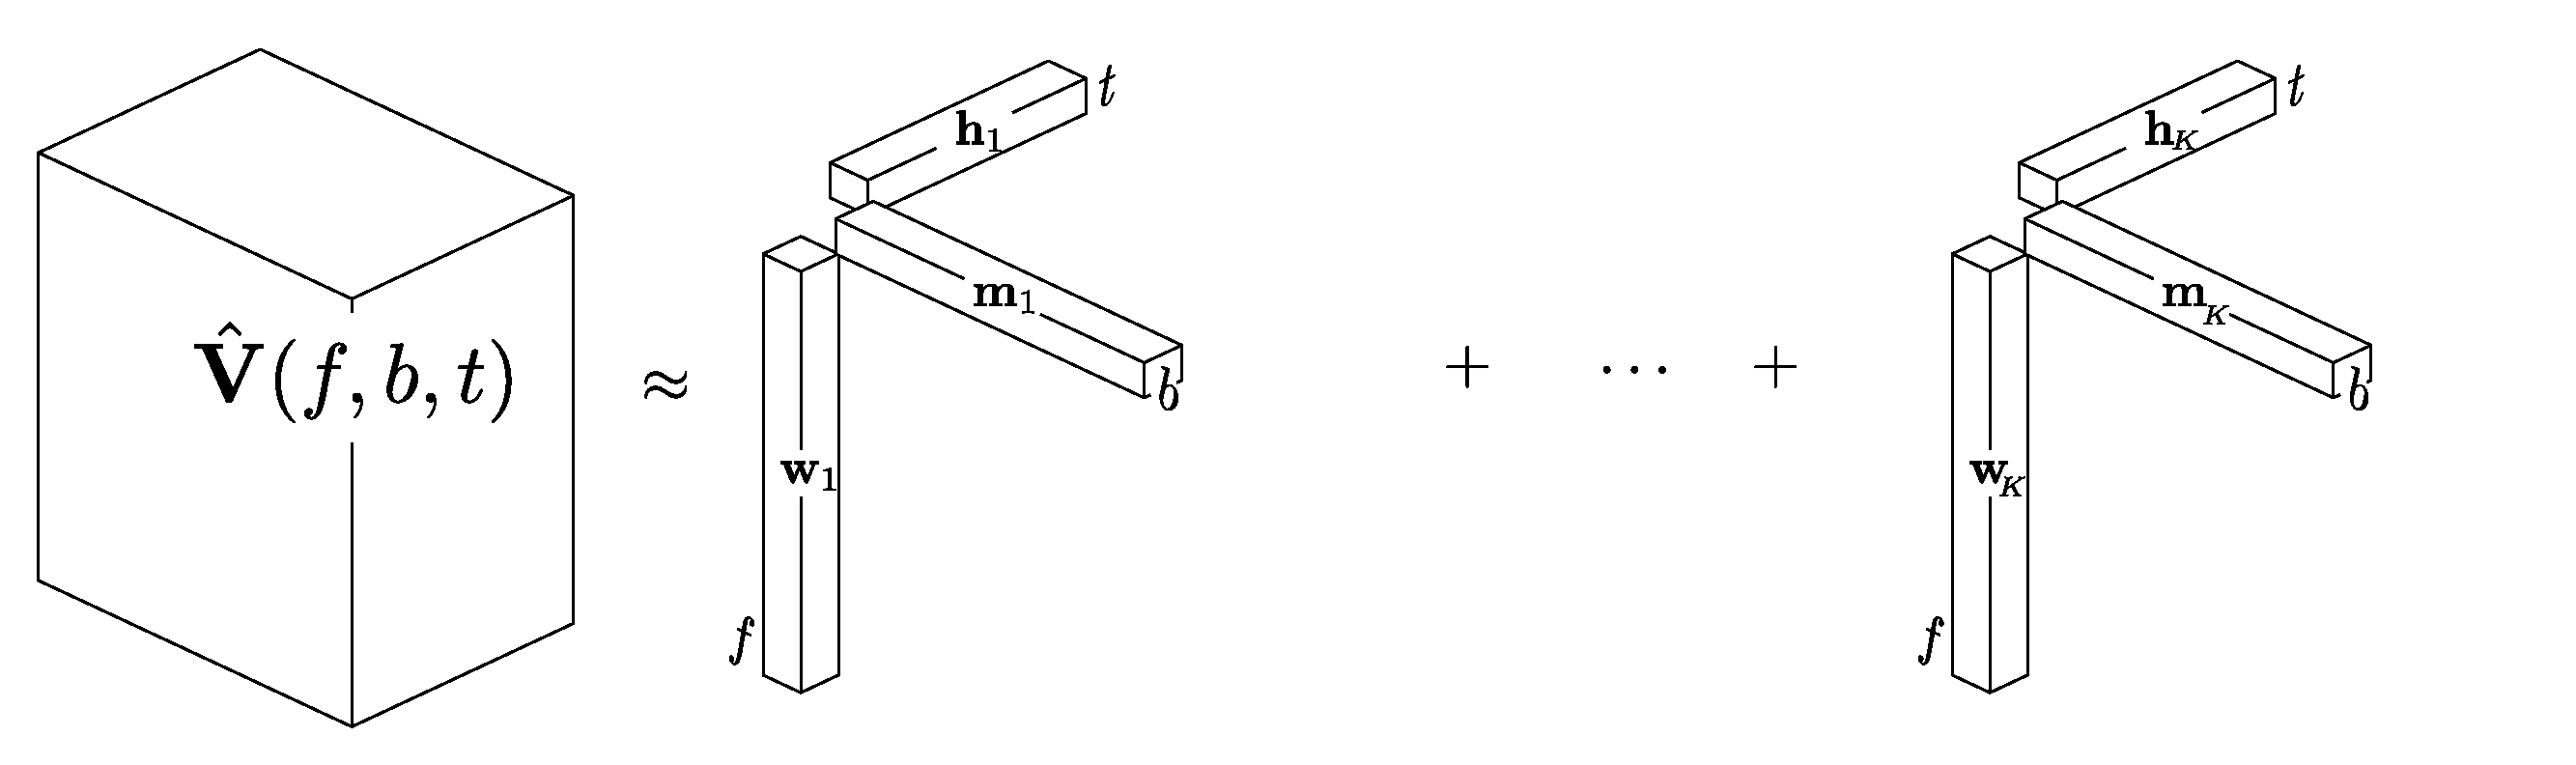
\includegraphics[width=0.8\textwidth]{Chapters/06_Separation_Unknown/figures/cpd.pdf}
  \caption{NMF }
  \label{fig:cpd}
\end{figure}


In the following subsection I will introduce the work of Barker and how it can be applied to the unison source separation problem.

%\from dafx
%%%%%%%%%%%%%%%%%%%%%%%%%%%%%%%%%%%%%%%%%%%%%%%%%%%%%%%%%%%%%%%%%%%%%%%%%%%%%%%%%
\section{Exploiting Amplitude Modulation using Tensor Factorizations}
\label{sub:am}

\marginpar{Parts of this subsection is also based on the work~\cite{stoeter14}.}


% Intro commonfate START
Since the vibrato does not only cause frequency modulation (FM) but also amplitude modulation (AM), so-called modulation spectra can be used to identify the modulation pattern. This is often calculated by taking the Fourier transform of a magnitude spectrum. Thus, the \emph{modulation spectrogram} has already gathered much attention in speech recognition~\cite{greenberg97,kingsbury98} and classification~\cite{kinnunen08, markaki09}.

% from zafar
Expanding NMF to tensors allows to incorporate more complex models, useful in many applications like multi-channel separation.
Extensions to NMF such as shift-invariance or convolutions were carried over to non-negative tensor (NTF) based algorithms~\cite{fitzgerald05, fitzgerald08, fitzgerald06, fevotte10, ozerov11}. 
These approaches, relying on decomposing mixtures of musical instruments, work well when certain assumptions hold to be true.

One way of analyzing it is the modulation spectrogram which is a frequency-frequency representation of a time domain input signal.
A complete signal representation can be archived by a modulation tensor which holds the modulation spectrograms for each time frame.
In practice, the modulation tensor \(\mathbf{V}_{f, b, t}\) can be computed from a the modulus of a time frequency matrix \(| \mathbf{X}_{f, t} |\) by computing \(f\) time frequency transforms over frequency band of \(\mathbf{X}\).

% TODO: add more info about how to form a modulation tensor for AM.
% the key point is that after the TF transform the magnitude has to be taken to compute the amplitude modulation. Computing the frequency modulation spectrogram is not possble in a simple way. WHY?

% Known modulation
The core intuition here is that one could observe that different amplitude modulation frequencies on certain frequency bands could be a distinct property of some instruments.
For example, if we mix together two harmonic signals having a fundamental frequency of 440Hz where one signal has a stationary amplitude modulation of 4~Hz and another one of 10~Hz, these differences are latent in a non-negative time frequency representation such as a time-frequency spectrogram.

Barker and Virtanen~\cite{barker13} were the first to propose a modulation tensor representation for single channel source separation. 
This work factorization on the tensor by using the well known PARAFAC/CANDECOMP (CP) decomposition~\cite{cichocki09, kolda09}.\\


\subsection{Non-Negative Tensor Factorization}

% TODO:
% we implemented a custom C++ version of the PARAFAC product.
% we included  Parallelisation, SIMD Vectorized and it is Cache Optimized
%
% Depending on the data size, between 20 and 40 times faster than a Python implementation of the same operation !  Also found that in the original algorithm, it is not necessary to perform
%
% this product for every factor, but only for each iteration !  This implementation can be used not only for Beta-NTF but also for
%
% many other algorithms using PARAFAC or CANDECOMP

NTF approximates a modulation tensor \(V\) by a product of three matrices containing the frequency/basis, time/activation signals, and the modulation gain for each component.
A very popular factorization model is called is the PARAFAC decomposition:

\begin{equation}
   \mathbf{V} \approx \sum\limits_{j=1}^{J} \mathbf{w}_{j}(f) \circ \mathbf{m}_{j}(b) \circ \mathbf{h}_{j}(t).
\end{equation}

where the \(\circ\) operator is usually called the CP product and is depicted in Figure~\ref{fig:cpd}.
For an introduction on matrix and tensor factorizations, the reader is referred to~\cite{cichocki09}.

Tensor factorization is often not consistent, please see~\cite{kolda09} for a unifying approach.

\begin{figure}
  \centering
  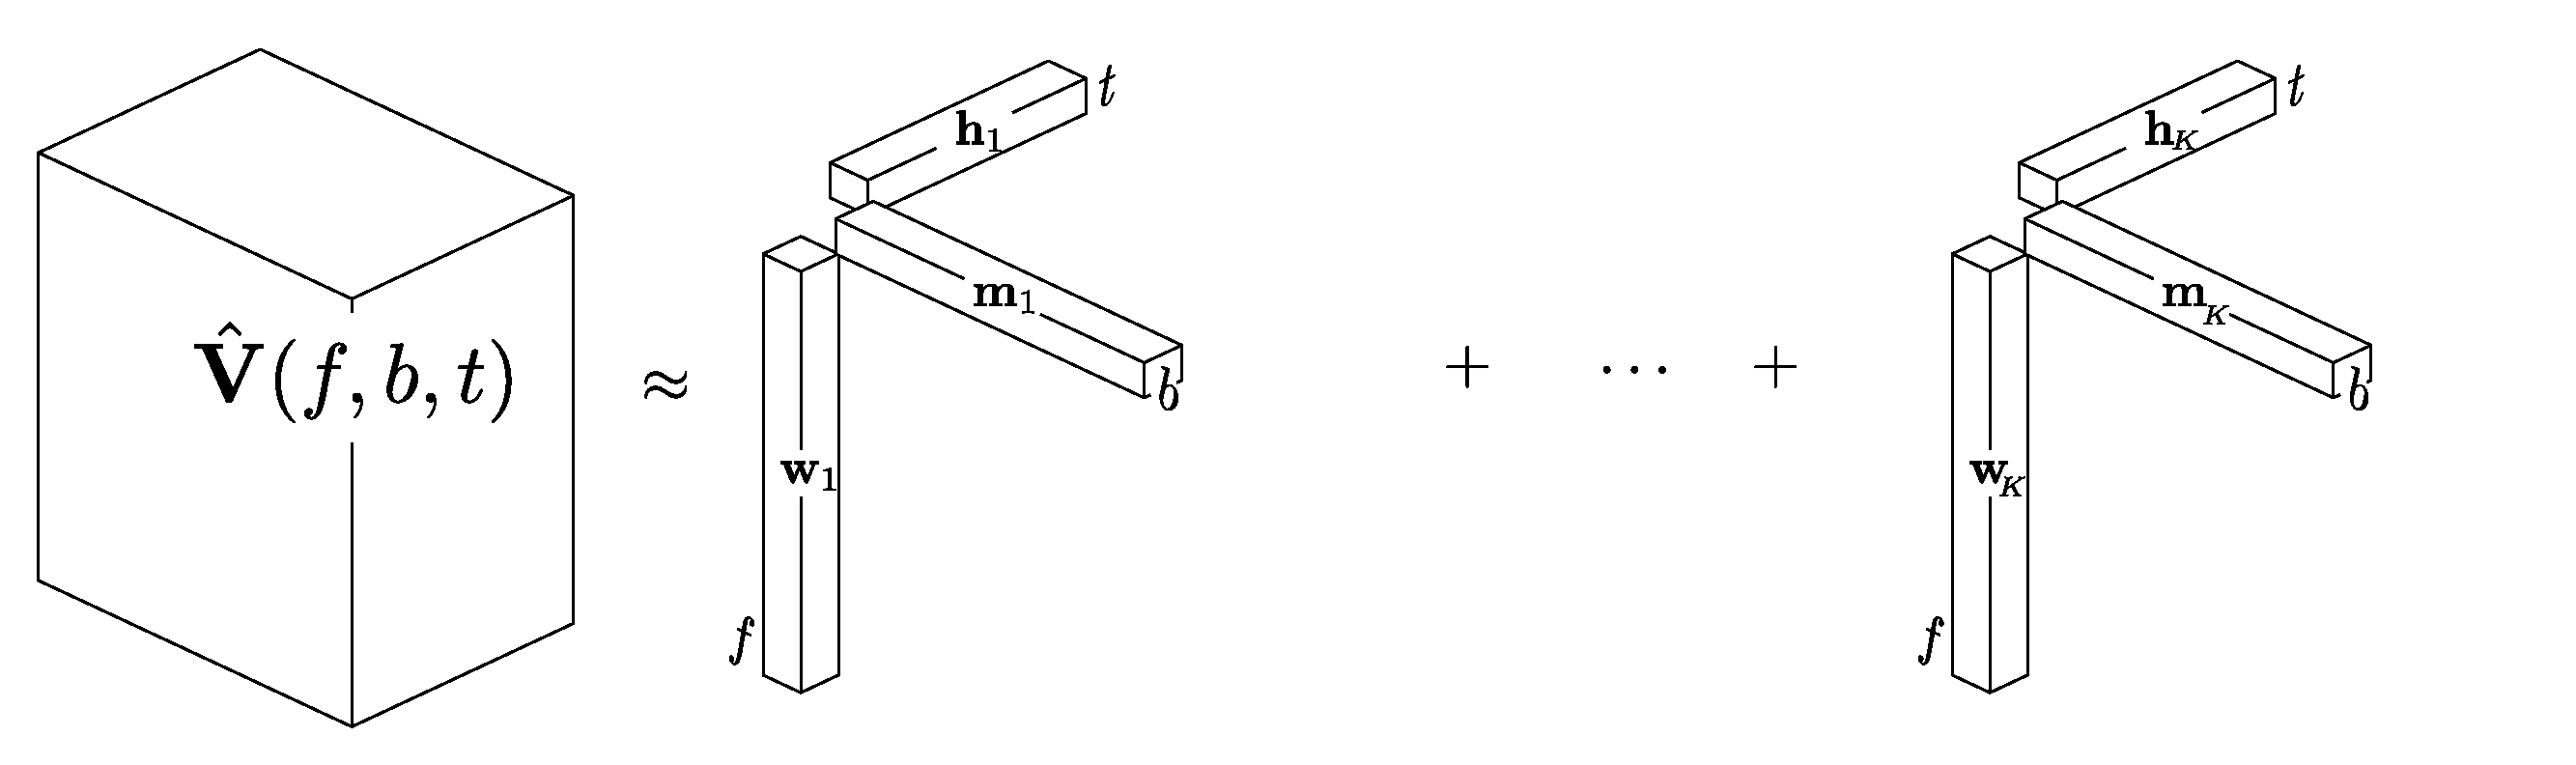
\includegraphics[width=0.8\textwidth]{Chapters/06_Separation_Unknown/figures/cpd.pdf}
  \caption{PARAFAC Decomposition in an example for a three-dimensional tensor \(mathbf{V}\) into three rank 1 vectors.}
  \label{fig:cpd}
\end{figure}
\par
Compared to~\cite{barker13} we choose to generate the modulation tensor in way that is simpler and easier to invert. Barker and Virtanen use a Gammatone filter bank and  rectification to model the characteristics of the human auditory system. We used a two-stage DFT filter bank where the modulation domain is based on  magnitude spectrograms. Although this can give perceptually less optimal results, each step can be directly inverted by using the complex representation. Barker already showed that the NTF based approach gives better results on speech signals. We found that this approach can be used to separate two instrument mixtures by their amplitude modulation characteristics and is therefore ideal for the unison scenario.

NTF gives a smoother activation matrix and is able to generate the output with the separated amplitude modulations on each sinusoid. The modulation frequency gain matrix shows the two modulation frequency templates and the DC-component.

\begin{figure}[h]
\centering
% \subcaptionbox{Time Domain}%
% [1\textwidth]{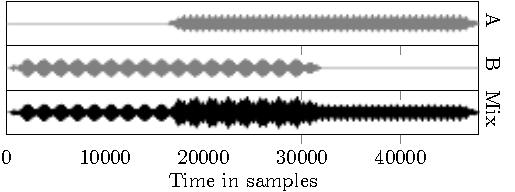
\includegraphics[width=0.8\textwidth]{Chapters/05_Separation_Known/figures/Timepdf-crop.pdf}}%
% \hspace{0.2\textwidth} % separation
\subcaptionbox{Slice of Modulation Tensor}
[1\textwidth]{% This file was created by matlab2tikz v0.4.7 (commit 3442858e5a642c135c5e9dab6a960bee5b9c6f8d) running on MATLAB 8.2.
% Copyright (c) 2008--2014, Nico Schlmer <nico.schloemer@gmail.com>
% All rights reserved.
% Minimal pgfplots version: 1.3
%
% The latest updates can be retrieved from
%   http://www.mathworks.com/matlabcentral/fileexchange/22022-matlab2tikz
% where you can also make suggestions and rate matlab2tikz.
%
\begin{tikzpicture}[font=\small]

\begin{axis}[%
width=0.73\textwidth,
height=3.5cm,
axis on top,
trim axis left,
scale only axis,
xmin=0.5,
xmax=81.5,
ymin=0.5,
ymax=137.5,
xlabel=Frames,
ylabel=Modulation Frequency Bins,
every axis y label/.style={at={(current axis.north east)},below=18mm,xshift=8mm},
y label style={rotate=-90},
]
\addplot [forget plot] graphics [xmin=0.5,xmax=81.5,ymin=0.5,ymax=137.5] {Chapters/05_Separation_Known/figures/AMPlots/Tmod-1_scaled.png};
\end{axis}
\end{tikzpicture}%
}%
\hspace{0.3\textwidth} % separation
\subcaptionbox{Tensor Factorization}
[1\textwidth]{% This file was created by matlab2tikz v0.4.7 (commit 3442858e5a642c135c5e9dab6a960bee5b9c6f8d) running on MATLAB 8.2.
% Copyright (c) 2008--2014, Nico Schlmer <nico.schloemer@gmail.com>
% All rights reserved.
% Minimal pgfplots version: 1.3
%
% The latest updates can be retrieved from
%   http://www.mathworks.com/matlabcentral/fileexchange/22022-matlab2tikz
% where you can also make suggestions and rate matlab2tikz.
%
\begin{tikzpicture}[font=\small]

\begin{axis}[%
width=0.15\columnwidth,
height=3.5cm,
axis on top,
xminorgrids=true,
minor xtick={1.5,2.5},
scale only axis,
xtick={1,2},
xmin=0.5,
xmax=2.5,
ymin=0.5,
ymax=137.5,
name=plot2,
xlabel=Gain Components,
ylabel=Modulation Frequency Bins,
every axis y label/.style={at={(current axis.north east)},below=18mm,xshift=8mm},
y label style={rotate=-90},
]
\addplot [forget plot] graphics [xmin=0.5,xmax=2.5,ymin=0.5,ymax=137.5] {Chapters/05_Separation_Known/figures/AMPlots/GAS-1_scaled.png};
\end{axis}

\begin{axis}[%
width=0.15\columnwidth,
height=3.5cm,
xminorgrids=true,
minor xtick={1.5,2.5},
axis on top,
scale only axis,
xtick={1,2},
xmin=0.5,
xmax=2.5,
ymin=0.5,
ymax=145.5,
xlabel=Basis Components,
ylabel=Frequency Bins,
every axis y label/.style={at={(current axis.north east)},below=18mm,xshift=8mm},
y label style={rotate=-90},
at=(plot2.left of south west),
anchor=right of south east
]
\addplot [forget plot] graphics [xmin=0.5,xmax=2.5,ymin=0.5,ymax=145.5] {Chapters/05_Separation_Known/figures/AMPlots/GAS-2_scaled.png};
\end{axis}

\begin{axis}[%
width=0.15\columnwidth,
height=3.5cm,
xminorgrids=true,
minor xtick={1.5,2.5},
axis on top,
scale only axis,
xtick={1,2},
xmin=0.5,
xmax=2.5,
ymin=0.5,
ymax=81.5,
xlabel=Activation Components,
ylabel=Frames,
every axis y label/.style={at={(current axis.north east)},below=18mm,xshift=8mm},
y label style={rotate=-90},
at=(plot2.right of south east),
anchor=left of south west
]
\addplot [forget plot] graphics [xmin=0.5,xmax=2.5,ymin=0.5,ymax=81.5] {Chapters/05_Separation_Known/figures/AMPlots/GAS-3_scaled.png};
\end{axis}
\end{tikzpicture}%
}%
\caption{\textbf{(a)} Modulation tensor slice of a mixture of two sinusoids at $440$ Hz with AM of $4.7$ Hz and $12.6$ Hz (sample rate=$8$ kHz)  (FFT length = 256), \textbf{(b)}  $\mathbf{G} \times \mathbf{A} \times \mathbf{S} $ Result of Non-Negative Tensor Factorization ($\beta = 1$) after 100 iterations}
\label{fig:count}
\end{figure}


% \begin{figure}[H]
%     \centering
%     \tiny
%     \subfloat[Input]{
%        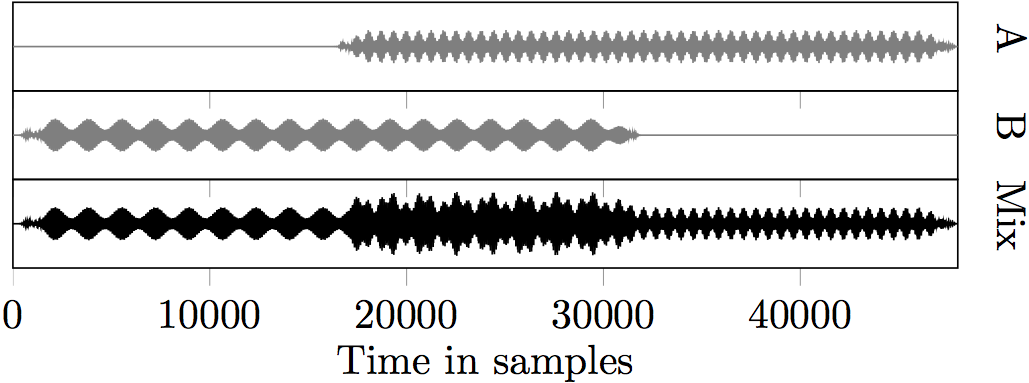
\includegraphics[width=0.8\columnwidth]{Chapters/05_Separation_Known/figures/Timepdf-crop.png}\hspace{-7mm}
%     }\hfill
%     \subfloat[Spectrogram]{
%        % This file was created by matlab2tikz% This file was created by matlab2tikz v0.4.7 (commit 3442858e5a642c135c5e9dab6a960bee5b9c6f8d) running on MATLAB 8.2.
% Copyright (c) 2008--2014, Nico Schlmer <nico.schloemer@gmail.com>
% All rights reserved.
% Minimal pgfplots version: 1.3
%
% The latest updates can be retrieved from
%   http://www.mathworks.com/matlabcentral/fileexchange/22022-matlab2tikz
% where you can also make suggestions and rate matlab2tikz.
%
\begin{tikzpicture}[font=\small]

\begin{axis}[%
width=0.225\columnwidth,
height=3.5cm,
axis on top,
xminorgrids=true,
minor xtick={1.5,2.5},
scale only axis,
xtick={1,2},
xmin=0.5,
xmax=2.5,
ymin=0.5,
ymax=137.5,
name=plot2,
xlabel=Gain Components,
ylabel=Modulation Frequency Bins,
every axis y label/.style={at={(current axis.north east)},below=18mm,xshift=4mm},
y label style={rotate=-90},
]
\addplot [forget plot] graphics [xmin=0.5,xmax=2.5,ymin=0.5,ymax=137.5] {Chapters/dafx/figures/AMPlots/GAS-1_scaled.png};
\end{axis}

\begin{axis}[%
width=0.225\columnwidth,
height=3.5cm,
xminorgrids=true,
minor xtick={1.5,2.5},
axis on top,
scale only axis,
xtick={1,2},
xmin=0.5,
xmax=2.5,
ymin=0.5,
ymax=145.5,
xlabel=Basis Components,
ylabel=Frequency Bins,
every axis y label/.style={at={(current axis.north east)},below=18mm,xshift=4mm},
y label style={rotate=-90},
at=(plot2.left of south west),
anchor=right of south east
]
\addplot [forget plot] graphics [xmin=0.5,xmax=2.5,ymin=0.5,ymax=145.5] {Chapters/dafx/figures/AMPlots/GAS-2_scaled.png};
\end{axis}

\begin{axis}[%
width=0.225\columnwidth,
height=3.5cm,
xminorgrids=true,
minor xtick={1.5,2.5},
axis on top,
scale only axis,
xtick={1,2},
xmin=0.5,
xmax=2.5,
ymin=0.5,
ymax=81.5,
xlabel=Activation Components,
ylabel=Frames,
every axis y label/.style={at={(current axis.north east)},below=18mm,xshift=4mm},
y label style={rotate=-90},
at=(plot2.right of south east),
anchor=left of south west
]
\addplot [forget plot] graphics [xmin=0.5,xmax=2.5,ymin=0.5,ymax=81.5] {Chapters/dafx/figures/AMPlots/GAS-3_scaled.png};
\end{axis}
\end{tikzpicture}%
 v0.4.7 (commit 3442858e5a642c135c5e9dab6a960bee5b9c6f8d) running on MATLAB 8.2.
% Copyright (c) 2008--2014, Nico Schlmer <nico.schloemer@gmail.com>
% All rights reserved.
% Minimal pgfplots version: 1.3
%
% The latest updates can be retrieved from
%   http://www.mathworks.com/matlabcentral/fileexchange/22022-matlab2tikz
% where you can also make suggestions and rate matlab2tikz.
%
\begin{tikzpicture}[font=\small]

\begin{axis}[%
    /pgf/number format/.cd,
           use comma,
           1000 sep={},
width=0.35\columnwidth,
height=3.5cm,
axis on top,
scale only axis,
xmin=0.5,
xmax=1497.5,
ymin=0.5,
ymax=145.5,
xlabel=Frames,
ylabel=Frequency Bins,
every axis y label/.style={at={(current axis.north east)},below=18mm,xshift=4mm},
y label style={rotate=-90},
]
\addplot [forget plot] graphics [xmin=0.5,xmax=1497.5,ymin=0.5,ymax=145.5] {Chapters/05_Separation_Known/figures/AMPlots/STFT-1_scaled.png};
\end{axis}
\end{tikzpicture}%
%
%     }%
%     \subfloat[Tensor Slice]{
%        % This file was created by matlab2tikz v0.4.7 (commit 3442858e5a642c135c5e9dab6a960bee5b9c6f8d) running on MATLAB 8.2.
% Copyright (c) 2008--2014, Nico Schlmer <nico.schloemer@gmail.com>
% All rights reserved.
% Minimal pgfplots version: 1.3
%
% The latest updates can be retrieved from
%   http://www.mathworks.com/matlabcentral/fileexchange/22022-matlab2tikz
% where you can also make suggestions and rate matlab2tikz.
%
\begin{tikzpicture}[font=\small]

\begin{axis}[%
width=0.73\textwidth,
height=3.5cm,
axis on top,
trim axis left,
scale only axis,
xmin=0.5,
xmax=81.5,
ymin=0.5,
ymax=137.5,
xlabel=Frames,
ylabel=Modulation Frequency Bins,
every axis y label/.style={at={(current axis.north east)},below=18mm,xshift=8mm},
y label style={rotate=-90},
]
\addplot [forget plot] graphics [xmin=0.5,xmax=81.5,ymin=0.5,ymax=137.5] {Chapters/05_Separation_Known/figures/AMPlots/Tmod-1_scaled.png};
\end{axis}
\end{tikzpicture}%
%
%     }\hfill
%
%     \subfloat[NMF]{
%      	% This file was created by matlab2tikz v0.4.7 (commit 3442858e5a642c135c5e9dab6a960bee5b9c6f8d) running on MATLAB 8.2.
% Copyright (c) 2008--2014, Nico Schlmer <nico.schloemer@gmail.com>
% All rights reserved.
% Minimal pgfplots version: 1.3
%
% The latest updates can be retrieved from
%   http://www.mathworks.com/matlabcentral/fileexchange/22022-matlab2tikz
% where you can also make suggestions and rate matlab2tikz.
%
\begin{tikzpicture}[font=\small]

\begin{axis}[%
/pgf/number format/.cd, use comma, 1000 sep={},
width=0.225\columnwidth,
height=3.5cm,
axis on top,
scale only axis,
xtick={1,2},
xminorgrids=true,
minor xtick={1.5},
xmin=0.5,
xmax=2.5,
ymin=0.5,
ymax=145.5,
name=plot1,
xlabel=Basis Components,
ylabel=Frequency Bins,
every axis y label/.style={at={(current axis.north east)},below=18mm,xshift=8mm},
y label style={rotate=-90},
]
\addplot [forget plot] graphics [xmin=0.5,xmax=2.5,ymin=0.5,ymax=145.5] {Chapters/05_Separation_Known/figures/AMPlots/WH-1_scaled.png};
\end{axis}

\begin{axis}[%
/pgf/number format/.cd, use comma, 1000 sep={},
width=0.225\columnwidth,
height=3.5cm,
axis on top,
scale only axis,
xminorgrids=true,
minor xtick={1.5},
xtick={1,2},
xmin=0.5,
xmax=2.5,
ymin=0.5,
ymax=1497.5,
xlabel=Activation Components,
ylabel=Frames,
every axis y label/.style={at={(current axis.north east)},below=18mm,xshift=8mm},
y label style={rotate=-90},
at=(plot1.right of south east),
anchor=left of south west
]
\addplot [forget plot] graphics [xmin=0.5,xmax=2.5,ymin=0.5,ymax=1497.5] {Chapters/05_Separation_Known/figures/AMPlots/WH-2_scaled.png};
\end{axis}
\end{tikzpicture}%
%
%     }\hfill
%     \subfloat[Non-Negative Tensor Factorization]{
%        % This file was created by matlab2tikz v0.4.7 (commit 3442858e5a642c135c5e9dab6a960bee5b9c6f8d) running on MATLAB 8.2.
% Copyright (c) 2008--2014, Nico Schlmer <nico.schloemer@gmail.com>
% All rights reserved.
% Minimal pgfplots version: 1.3
%
% The latest updates can be retrieved from
%   http://www.mathworks.com/matlabcentral/fileexchange/22022-matlab2tikz
% where you can also make suggestions and rate matlab2tikz.
%
\begin{tikzpicture}[font=\small]

\begin{axis}[%
width=0.15\columnwidth,
height=3.5cm,
axis on top,
xminorgrids=true,
minor xtick={1.5,2.5},
scale only axis,
xtick={1,2},
xmin=0.5,
xmax=2.5,
ymin=0.5,
ymax=137.5,
name=plot2,
xlabel=Gain Components,
ylabel=Modulation Frequency Bins,
every axis y label/.style={at={(current axis.north east)},below=18mm,xshift=8mm},
y label style={rotate=-90},
]
\addplot [forget plot] graphics [xmin=0.5,xmax=2.5,ymin=0.5,ymax=137.5] {Chapters/05_Separation_Known/figures/AMPlots/GAS-1_scaled.png};
\end{axis}

\begin{axis}[%
width=0.15\columnwidth,
height=3.5cm,
xminorgrids=true,
minor xtick={1.5,2.5},
axis on top,
scale only axis,
xtick={1,2},
xmin=0.5,
xmax=2.5,
ymin=0.5,
ymax=145.5,
xlabel=Basis Components,
ylabel=Frequency Bins,
every axis y label/.style={at={(current axis.north east)},below=18mm,xshift=8mm},
y label style={rotate=-90},
at=(plot2.left of south west),
anchor=right of south east
]
\addplot [forget plot] graphics [xmin=0.5,xmax=2.5,ymin=0.5,ymax=145.5] {Chapters/05_Separation_Known/figures/AMPlots/GAS-2_scaled.png};
\end{axis}

\begin{axis}[%
width=0.15\columnwidth,
height=3.5cm,
xminorgrids=true,
minor xtick={1.5,2.5},
axis on top,
scale only axis,
xtick={1,2},
xmin=0.5,
xmax=2.5,
ymin=0.5,
ymax=81.5,
xlabel=Activation Components,
ylabel=Frames,
every axis y label/.style={at={(current axis.north east)},below=18mm,xshift=8mm},
y label style={rotate=-90},
at=(plot2.right of south east),
anchor=left of south west
]
\addplot [forget plot] graphics [xmin=0.5,xmax=2.5,ymin=0.5,ymax=81.5] {Chapters/05_Separation_Known/figures/AMPlots/GAS-3_scaled.png};
\end{axis}
\end{tikzpicture}%
%
%     }\hfill
%     \caption{Example of separating a mixture of two amplitude modulated signals by NMF and Modulation-NTF. \\ \textbf{(a)} Mixture of two sinusoids at $440$ Hz with AM of $4.7$ Hz and $12.6$ Hz (fs=$8$ kHz), \textbf{(b)} STFT (FFT length = 256), \textbf{(c)} Slice of Modulation Tensor (FFT length = 256),  \textbf{(d)} $\mathbf{W} \times \mathbf{H}$ Result of Non-Negative Matrix Factorization ($\beta = 1$) after 100 iterations, \textbf{(e)}  $\mathbf{G} \times \mathbf{A} \times \mathbf{S} $ Result of Non-Negative Tensor Factorization ($\beta = 1$) after 100 iterations,}
%     \label{fig:am_tensor}
% \end{figure}

A comparison of the modulation tensor approach in the context of unison separation has been carried out in our work published in~\cite{stoeter14}.

Furthermore in that work, we also compared to the pitch variation informed method, presented in the previous chapter.
Results indicated that modulation tensor factorization approach work on some instruments mixtures but not generally.
The reason is that, that it does only consider amplitude modulation even though frequency modulations are the actual source of modulation.
In the next section we therefore investigated how the complex modulation that consist of both, frequency and amplitude modulation patterns caused by the instrument vibratos, can be utilized.

\section{Exploiting General Modulation Textures}

\marginpar{This section is based on the work that has been published in 2016~\cite{stoeter16}. The work has been done in collaboration with Antoine Liutkus (INRIA, France) and Roland Badeau (ParisTech, France).}

In this work we introduce a novel tensor signal representation which additionally exploits similarities in the frequency direction.
We can therefore make use of dependencies between modulations of neighboring bins.
This is similar to the recently proposed High-Resolution Nonnegative Matrix Factorization model that accounts for dependencies in the time-frequency plane (HR-NMF~\cite{badeau11}).
In short, HR-NMF models each complex entry of a time-frequency transform of an audio signal as a linear combination of its neighbors, enabling the modeling of damped sinusoids, along with an independent innovation.
This model was generalized to multichannel mixtures in~\cite{badeau13a,badeau14} and was shown to provide considerably better oracle performance for source separation than alternative models in~\cite{magron15a}.
Indeed, even though some variational approximations were introduced in~\cite{badeau13} to strongly reduce their complexity, those algorithms are often demanding for practical applications.
In this work, we proposed to relax some assumptions of HR-NMF in the interest of simplifying the estimation procedure.
The core idea is to divide the complex spectrogram into modulation patches in order to group common modulation in time and frequency direction.
We call this the \emph{Common Fate Model} (CFM), borrowing from the Gestalt theory, which describes how human perception merges objects that move together over time.
Bregman~\cite{bregman94} described the Common Fate theory for auditory scene analysis as the ability to group sound objects based on their common motion over time, as occurs with frequency modulations of harmonic partials.
As outlined by Bregman, the human ability to detect and group sound sources by small differences in FM and AM is outstanding.
Also, it turns out that humans are especially sensitive to modulation frequencies around 5~Hz, which is the typical vibrato frequency that many musicians produce naturally.
% TODO add more gestalt stuff, maybe the image.
% Intro commonfate END

\subsection{The Common Fate Transform}
\label{sub:CFT}s

Let $\tilde{x}$ denote a single channel audio signal.
Its Short-Term Fourier Transform (STFT) is computed by splitting it into overlapping frames, and then taking the discrete Fourier transform (DFT) of each one.
Since the waveform~$\tilde{x}$ is real, the Fourier transform of
each frame is Hermitian. In the following, we assume that the redundant
information has been discarded to yield the STFT.
The resulting information is gathered into an $N_{\omega}\times N_{\tau}$
matrix written~$X$, where~$N_{\omega}$ is the number of frequency
bands and $N_{\tau}$ the total number of frames.
%
In this study, we will consider the properties of another object, built from $X$, which we call the Common Fate Transform (CFT).
It is constructed as illustrated in Figure~\ref{fig:CFT}.
We split the STFT~$X$ into overlapping rectangular $N_{a}\times N_{b}$ patches, regularly spaced over both time and frequency.
For reference later in this thesis, we will call this representation the \emph{Grid STFT} (GFT).
Then, the 2D-DFT of each patch is computed\footnote{Note that since each patch is complex, its 2D-DFT is not Hermitian, thus all its entries are kept.}.
This yields an $N_{a}\times N_{b}\times N_{f}\times N_{t}$ tensor we write~$x$, where~$N_{f}$ and~$N_{t}$ are the vertical and horizontal positions for the patches, respectively.

As can be seen, the CFT is basically a further short-term 2D-DFT taken over the standard STFT~$X$.
One of the main differences compared to modulation spectrograms is that the CFT is computed using the complex STFT~$X$, and not a magnitude representation such as $\left|X\right|$.
As we will show, this simple difference has many interesting consequences, notably that the CFT is invertible: the original waveform~$\tilde{x}$ can be exactly recovered by cascading two classical overlap-add procedures.
Another difference is that the patches span several frequency bins, \emph{i.e.} we may have~$N_{a}>1$.
This contrasts with the conventional modulation spectrogram, that is usually defined using one frequency band only.

\begin{figure}[t]
\centering
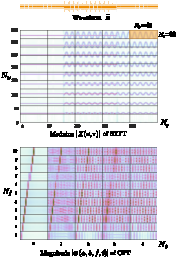
\includegraphics[width=0.8\textwidth]{Chapters/06_Separation_Unknown/figures/CFT}

\caption{Common Fate Transform. For convenience, the splitting of the STFT
into patches has been depicted without overlap, but overlapping patches
are used in practice\label{fig:CFT}.}
\end{figure}

\subsubsection{A Probabilistic Model for the CFT}

\label{ssub:separation}

When processing an audio signal~$\tilde{x}$ for source separation,
it is very common to assume that all time-frequency (TF) bins
of its STFT are independent~\cite{fevotte09, duong10, ozerov12, liutkus11t}.
This is often the consequence of two different assumptions.
The first one is to consider that all frames are independent, thus
leading to the independence of all entries of the STFT that do not belong to the
same column. The second one is related to the notion of stationarity:
roughly speaking, the Fourier transform is known to decompose stationary
signals into independent components, whether these signals be Gaussian
(see, e.g.~\cite{liutkus11t}) or, more generally, harmonisable.
As a consequence, when the signals are assumed to be \emph{locally stationary},
it is theoretically sound to assume that all the entries of
their STFT are independent.

Still, both assumptions can only be considered as approximations.
First, adjacent frames are obviously not independent, notably because
of the overlap between them. Second, the stationarity assumption is
only approximate in practice, especially when impulsive elements are
found in the audio, leading to strong dependencies among the different
frequency bins. Let $\{ X_{ft}\} _{f,t}$
denote all the $N_{a}\times N_{b}$ patches taken on the STFT to compute
the CFT, as depicted in Figure~\ref{fig:CFT}. The probabilistic
model we choose is the combination of \emph{three} different assumptions
made on the distribution of these patches.

\begin{enumerate}[leftmargin=0cm,itemindent=.5cm,labelwidth=\itemindent,labelsep=0cm,align=left]
\item All patches are independent. Just as the classical locally stationary
model~\cite{liutkus11t} assumes independence of overlapping frames,
we assume here independence of overlapping patches. Due to the
overlap between them, this assumption is an approximation,
and one may wonder what the advantage is of dropping independent frames
for independent patches. The answer lies in the fact that the latter
permits us to model phase dependencies between neighboring STFT entries,
and also to model much longer-term dependencies, as required for instance
by deterministic damped or frequency-modulated sinusoidal signals.\label{enu:assumption_independent_patches}
\item Each patch is \emph{stationary}: its distribution
is assumed invariant under translations in the TF plane. This is where we do not assume independence, but on the contrary expect dependencies among neighboring STFT entries. Our approach assumes this happens in a way that only depends on the relative positions in
the TF plane. It can easily be shown that mixtures of
damped sinusoids have this property. Assuming stationarity not only over time but over both time and frequency
also permits us to naturally account for mixtures of frequency-modulated
sounds. In short, we assume that throughout each patch, we observe
one coherent STFT ``texture''. The difference with the HR-NMF model is that we have independent and identically
distributed (i.i.d.) innovations for one given patch, whereas HR-NMF model has more variability and permits heteroscedastic innovations. However, taking overlapping patches somehow compensates for
this limitation.\label{enu:assumption_stationary}
% \item The joint distribution of all entries of each patch is $\alpha$-stable~\cite{samoradnitsky94}.
% $\alpha$-stable distributions are the only ones that are stable under additions, \emph{i.e.} such that
% sums of $\alpha$-stable random variables (r.v.) remain $\alpha$-stable.
% They notably comprise the Gaussian and Cauchy distributions as special
% cases when $\alpha=2$ and $\alpha=1$, respectively.\label{enu:assumption_alpha_stable}
\item Each patch is harmonisable, \emph{i.e.} is the inverse Fourier
transform of a complex random measure with independent increments.
In other words, all entries of the Fourier transform of each patch
are assumed to be asymptotically independent, as the size of the patch
gets larger. This rather technical condition, often tacitly made in
signal processing studies, permits efficient processing in the frequency
domain.\label{enu:assumption_harmonisable}
\end{enumerate}

Under those assumptions, all entries of the CFT~$x$ are independent
(assumptions~\ref{enu:assumption_independent_patches} and~\ref{enu:assumption_stationary}),
% and each one is distributed with respect to a complex isotropic $\text{\ensuremath{\alpha}}$-stable
% distribution, noted $S\alpha S_{c}$ (assumptions~\ref{enu:assumption_alpha_stable}
and~\ref{enu:assumption_harmonisable}\footnote{This result is the direct generalization
of~\cite[th. 6.5.1]{samoradnitsky94} to multi-dimensional stationary processes.}):
\begin{equation}
x\left(a,b,f,t\right)\sim S S_{c}\left(P\left(a,b,f,t\right)\right),\label{eq:SaS_model}
\end{equation}
where $P$ is a nonnegative $N_{a}\times N_{b}\times N_{f}\times N_{t}$
tensor that we call the \emph{modulation density}. In
the general case, it can basically be understood as the energy found at $\left(a,b\right)$ for patch
$\left(f,t\right)$, just like more classical (fractional) power spectral
densities describe the spectro-temporal energy content of the STFT
of a locally stationary signal.

\subsubsection{Another interpretation of the CFT}

\label{sub:interpretation}

An alternative interpretation of the CFT can be obtained by regarding the 2D-DFT
as two subsequent 1D-DFTs. If the transform in frequency direction (DFT-F) is
applied first, it is equivalent to a partial inverse DFT plus time reversal. If
the time reversal would be undone and an overlap-add would be applied, the
output would correspond to a subband representation with a frequency resolution
of $N_\omega / N_a$. Each of the $N_a$ final transformations (DFT-T) in one
patch takes output values from $N_b$ DFT-Ts with equal indices. This corresponds
to a splitting into poly-phase components with downsampling factor $N_a$ of the
time signal obtained by placing the output frames from the DFT-Ts in a row.
Thus, the outputs of the DFT-Fs have a very high frequency resolution of
$N_\omega N_b$ but contain aliasing components from the downsampling.

This interpretation of the CFT gives some indications for its benefits in the
separation of modulated sources. Due to the poly-phase representation it has a
relatively high temporal resolution. The periodicities in the spectra caused
by downsampling make the CFT relatively independent of frequency shifts, so
that, for example, the output patch of a single sinusoidal sweep is mainly
influenced by the sweep rate.

% todo add complexity analaysis

\subsection{Signal Separation}
Now, let us assume that the observed waveform is actually the sum
of~$J$ underlying sources~$\{ \tilde{s}_{j}\} _{j=1,\dots,J}$.
Due to the linearity of the CFT, this can be
expressed in the CFT domain as:
$$
\forall\left(a,b,f,t\right),x\left(a,b,f,t\right)=\sum\nolimits_{j}s_{j}\left(a,b,f,t\right).
$$
If we adopt the model presented above for each source
and use the stability property, we have:
$$
x\left(a,b,f,t\right)\sim S S_{c}\left(\sum\nolimits_{j}P_{j}\left(a,b,f,t\right)\right),
$$
where $P_{j}$ is the modulation density for source~$j$.
If these objects are known, it can be shown that each source can be
estimated in a maximum a posteriori sense from the mixture as:
\begin{equation}
\mathbb{E}\left[s_{j}\left(a,b,f,t\right)\mid \{ P_{j}\} _{j},x\right]=\tfrac{P_{j}\left(a,b,f,t\right)}{\sum_{j'}P_{j'}\left(a,b,f,t\right)} \, x\left(a,b,f,t\right)\label{eq:alpha_wiener}
\end{equation}
which we call the Wiener filter in~\cite{liutkus15}.
The resulting waveforms are readily obtained by inverting the CFT.\@
As can be seen, we now need to estimate the modulation
densities~$\{ P_{j}\} _{j}$ based on the observation
of the mixture CFT~$x$, similarly to the estimation of
 the sources' Power Spectral Densities (PSD)
in source separation studies.

\subsubsection{Factorization Model and Parameter Estimation}
\label{sub:NTF}

In order to estimate the sources' modulation densities, we first impose
a factorization model over them, so as to reduce the number of parameters
to be estimated. In this study, we set:
\begin{equation}
P_{j}\left(a,b,f,t\right)=A_{j}\left(a,b,f\right)H_{j}\left(t\right),\label{eq:NTF_model}
\end{equation}
where $A_{j}$ and $H_{j}$ are $N_{a}\times N_{b}\times N_{f}$ and~$N_{t}\times1$
nonnegative tensors, respectively. We call this a \emph{Common Fate
Model}. Intuitively, $A_{j}$ is a modulation density template that
is different for each frequency band~$f$, and that captures the
long term modulation profile of source~$j$ around that frequency.
Then, $H_{j}$ is an activation vector that indicates the strength
of source~$j$ on the patches located at temporal position~$t$.

% TODO: we also experiment with a, b * f * t with worse results. This means that the modulation tensor is not frequency independent.

% TODO: All patches are independent? Wie passt das zusammen?

% TODO: Explain that for N-way  arrays  with

Learning those parameters can be achieved using the conventional Nonnegative
Tensor Factorization methodology (see e.g.~\cite{cichoki09,ozerov12,smaragdis14}
for an overview and~\cite{liutkus15b} for the fitting of $S S_{c}$
parameters), except that it is applied to the CFT instead of the STFT,
and that the particular factorization to be used is~\eqref{eq:NTF_model}.
The factorization model is depicted in Figure~\ref{fig:cfm}

\begin{figure}[h]
\centering
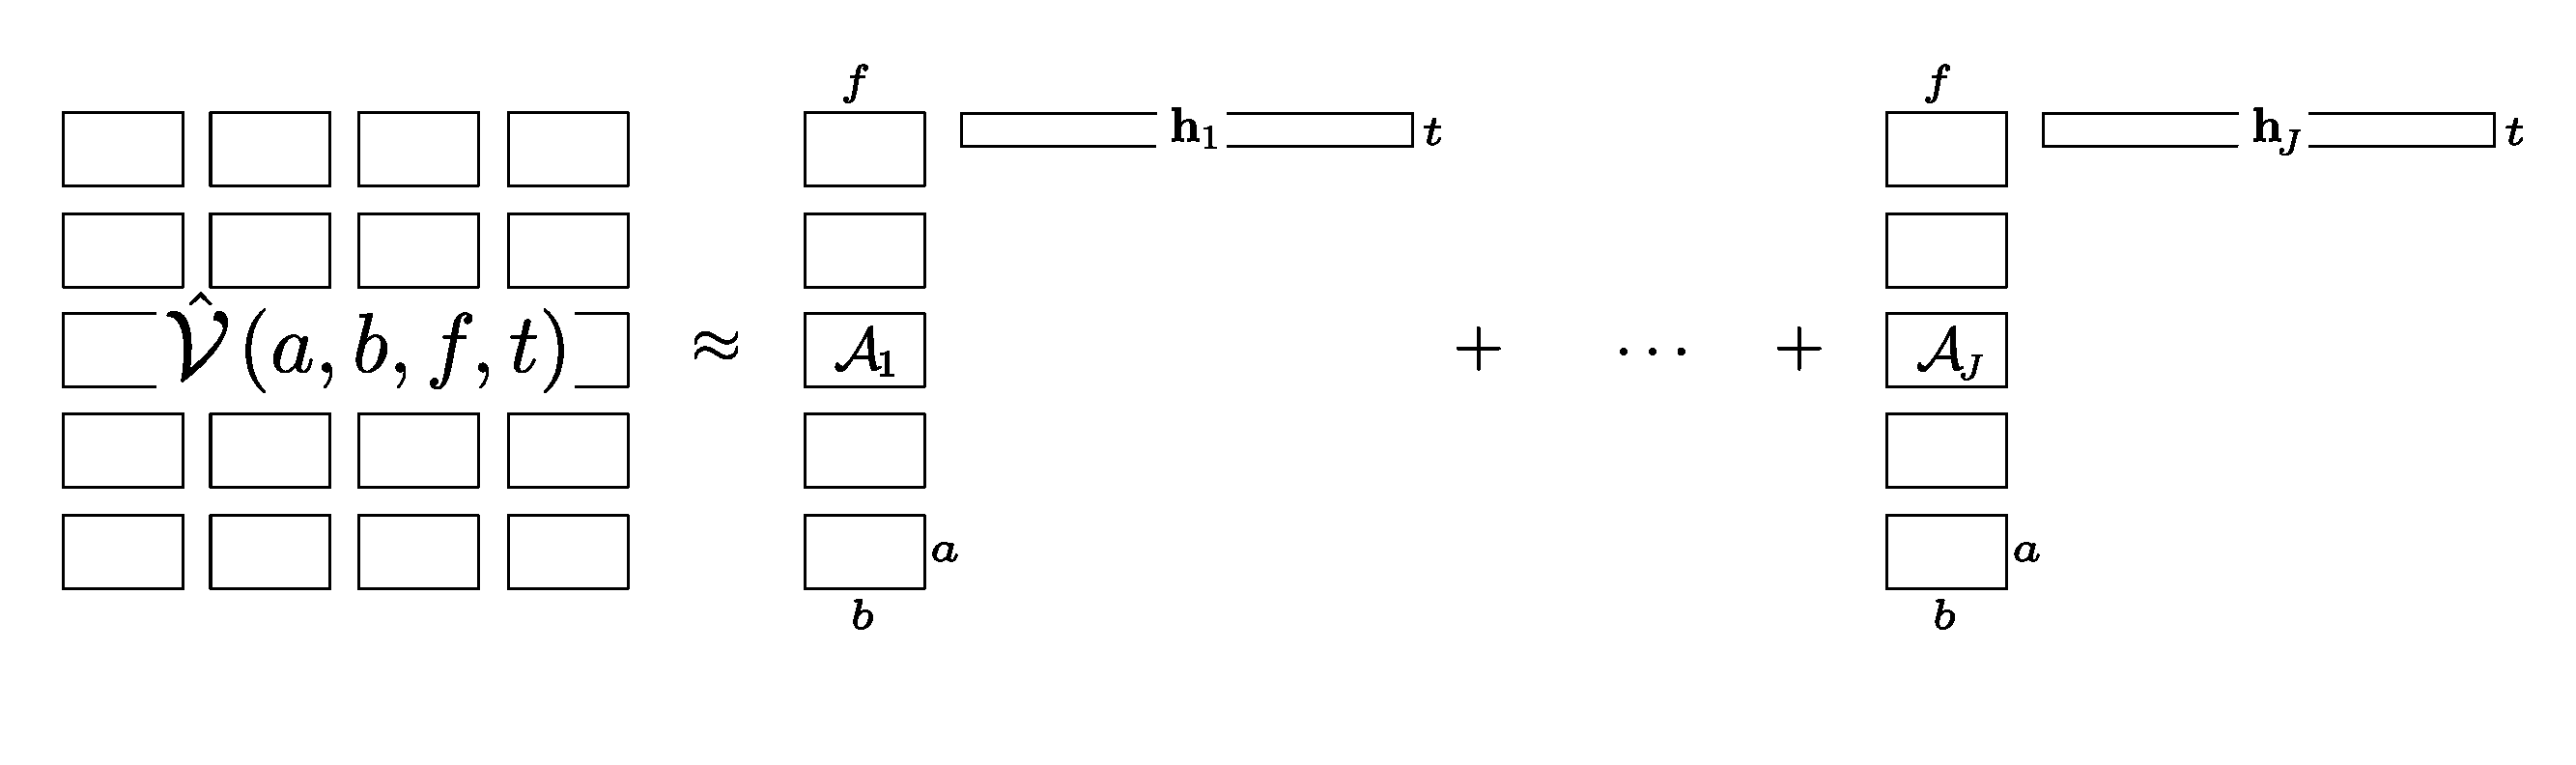
\includegraphics[width=0.8\textwidth]{Chapters/06_Separation_Unknown/figures/cfm.pdf}
\caption{Common Fate Model.}
\label{fig:cfm}
\end{figure}

In essence, it amounts to estimating the parameters~$\{ A_{j},H_{j}\} $
so that the modulus of the CFT is
as close as possible to~$\sum_{j}P_{j}$, with some particular
cost function as a data-fit criterion, called a $\beta$-divergence
and which includes Euclidean, Kullback-Leibler and Itakura-Saito as
special cases~\cite{fitzgerald08a}. As usual in such nonnegative models,
each parameter is updated in turn, while the others are kept fixed.
We provide the multiplicative updates in Algorithm~\ref{alg:Fitting-NTF}.
After a few iterations, the parameters can be used in~\eqref{eq:alpha_wiener} to separate
the sources.

\begin{algorithm}
With $v=\left|x\right|$ and always using the latest
parameters available for computing
 $\hat{P}\left(a,b,f,t\right)=\sum\limits_{j=1}^{J}A_{j}\left(a,b,f\right)H_{j}\left(t\right)$,
iterate:
\[
A_{j}\left(a,b,f\right)\leftarrow A_{j}\left(a,b,f\right)\tfrac{\sum_{t}v\left(a,b,f,t\right)\hat{P}\left(a,b,f,t\right)^{\cdot\left(\beta-2\right)}H_{j}\left(t\right)}{\sum_{t}\hat{P}\left(a,b,f,t\right)^{\cdot\left(\beta-1\right)}H_{j}\left(t\right)}
\]
\[
H_{j}\left(t\right)\leftarrow H_{j}\left(t\right)\tfrac{\sum_{a,b,f}v\left(a,b,f,t\right)\hat{P}\left(a,b,f,t\right)^{\cdot\left(\beta-2\right)}A_{j}\left(a,b,f\right)}{\sum_{a,b,f}\hat{P}\left(a,b,f,t\right)^{\cdot\left(\beta-1\right)}A_{j}\left(a,b,f\right)}.
\]


\caption{Fitting NMF parameters of the nonnegative CFM~\eqref{eq:NTF_model}.\label{alg:Fitting-NTF}}
\end{algorithm}

%!TEX root = ../icassp2016.tex
\subsection{Experiments}
\label{sec:experiment}

\begin{table*}[ht!]
  \centering
  \scriptsize
\begin{tabular}{ llll }
    \toprule
    Method & Signal Representation & Factorization Model \\
    \midrule
    CFM~\cite{stoter16} & STFT $\rightarrow$ Grid Slicing $\rightarrow$ 2D-DFT & $V(a,b,f,t) = P(a,b,f)\times H(t)$ \\
    NMF~\cite{virtanen07} & STFT & $V(f,t) = W(f)\times H(t)$ \\
    HR-NMF~\cite{badeau13} & Output of any filterbank (STFT, MDCT, \ldots)  & AR filtering of NMF excitation \\
    MOD~\cite{barker13} & STFT $\rightarrow$ $|\ldots|$ $\rightarrow$ STFT along each bin & $V(f,m,t) = W(f)\times A(m)\times H(t)$ \\
    CFMM & STFT $\rightarrow$ $|\ldots|$ $\rightarrow$ Grid Slicing $\rightarrow$ 2D-DFT & $V(a,b,f,t) = P(a,b,f)\cdot H(t)$ \\
    CFMMOD & STFT $\rightarrow$ $|\ldots|$ $\rightarrow$ Grid Slicing $\rightarrow$ 2D-DFT & $V(a,b,f,t) = P(a,b,f)\cdot H(t)$ \\
    \bottomrule
\end{tabular}
\caption{Overview of the evaluated algorithms}
\label{tab:methods}
\end{table*}

In this section, we present separation experiments utilizing CFM and compare it with other methods.

\subsubsection{Synthetic Example}
\label{sub:Synthentic_Examples}

To illustrate the CFT representation we processed a mixture consisting of two sinusoidal sources. One source is a pure sine wave of fundamental frequency 440~Hz whereas the other is frequency modulated by a sinusoid of 6.3~Hz. In the first step an STFT with a DFT-length of 1024 samples and a hop-size of 256 samples was processed at a sample rate of 22.05~kHz. Patches of size $(N_a, N_b) = (32, 48)$ (not respecting overlaps) were then taken from the STFT output. Figure~\ref{fig:CFT} in Section~\ref{sub:CFT} then shows the Common Fate Transform for the mixture as described in Section~\ref{sec:model}. One can see that the CFT representation shows distinct patterns across time, suggesting that the factorization is able to separate the sources.

% \begin{figure}[b]
% \centering
% 		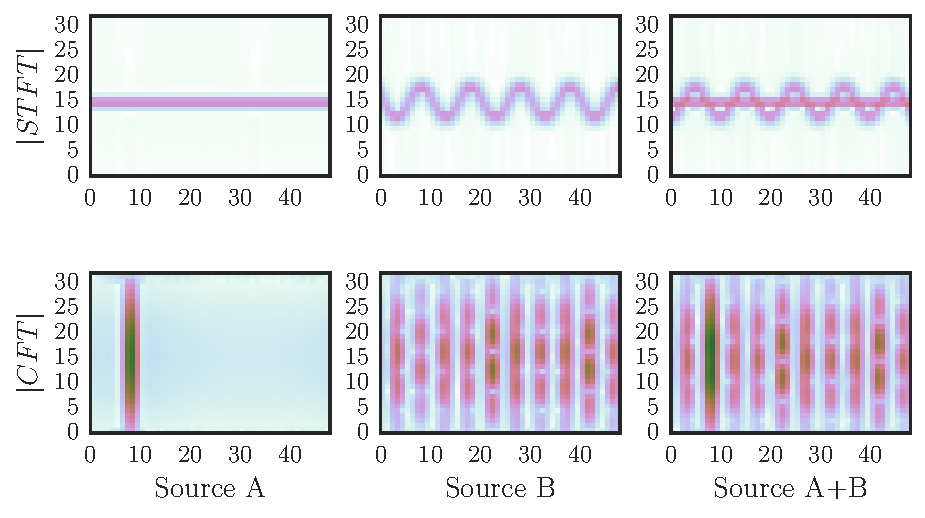
\includegraphics[width=0.8\textwidth]{Chapters/06_Separation_Unknown/figures/gridplot.pdf}
% \caption{Examples of patches of size $(N_a, N_b) = (32, 48)$. The upper row shows magnitude values from the STFT output, the lower row the corresponding Common Fate Transform (CFT).}
% \label{fig:gridplot}
% \end{figure}

\subsubsection{Objective Evaluation on Unison Instrument Mixtures}

For an evaluation of the method, we selected five musical instruments' samples, all featuring vibrato: violin, cello, tenor sax, English horn, and flute. It is important to note that vibrato techniques differ between instruments: whereas the English horn and the flute only produce a very subtle modulation, the violin and tenor sax have powerful frequency modulations with a higher modulation frequency as well as a higher modulation index. The signals have each been generated by rendering C4 (261.63~Hz) notes in a state-of-the-art software sampler\footnote{\textsc{Vienna Symphonic Library} (\url{https://vsl.co.at})}. All samples last about three seconds. We then generated a combination of ten mixtures of two instruments each, each one generated with a simple SourceA --- SourceB --- (SourceA + SourceB) scheme. Data were encoded in 44.1 kHz / 16 bit.
For evaluation, we compared separation performance of six different methods, summarized in Table~\ref{tab:methods}:
\begin{description}[style=unboxed,leftmargin=0cm]
\item[CFM] For the CFM model, we took an STFT with frames of 1024 samples and a hop-size of 512 samples. The resulting complex spectrogram was then split into a grid of patches of size $(N_a, N_b) = (4, 64)$, each having a half-window overlap in both dimensions.
\item[MOD] We implemented a modified version of~\cite{barker13} where for the sake of comparability, we used a STFT instead of a gammatone filterbank. A DFT length of 1024 and a hop-size of 512 samples were chosen. After taking the magnitude value, a second STFT of size 32 and hop-size 16 samples was computed for each frequency.
\item[CFMMOD] We selected patch sizes of $(N_a, N_b) = (1, 64)$ and modified the representation so that the magnitude spectrogram was used before computing the 2D-DFT.\@ This permits to compare the advantage of our proposed factorization model~(\ref{eq:NTF_model}) over MOD, when using the same kind of energy-modulation representation in both cases.
\item[CFMM] For comparing the influence of computing modulations over complex STFT or magnitude spectrograms, we tried our factorization model when the magnitude of the STFT is taken before 2D-DFT, with patches of the same size as for the CFM method.
\item[NMF] We took a standard NMF based method~\cite{virtanen07}. We highlight that taking a spectrogram with frames of length 1024 would not make a fair comparison, because the CFM model actually results in a larger frequency resolution. Therefore a comparable NMF is based on an STFT of DFT-length 32768.
\item[HR-NMF] See description in~\cite{magron15a}.
\end{description}
All factorizations ran for 100 iterations and were repeated five times. We chose $j=(2\ldots6)$ components for each factorization. For $j > 2$ we used oracle clustering to show the upper limit of SDR which can be achieved.

We ran the performance evaluation by using BSSeval~\cite{vincent06}. The results of Signal to Distortion
Ratio (SDR), Signal to Interference Ratio (SIR), and Signal to Artifacts Ration (SAR) are depicted in Figure~\ref{fig:boxplot_overall}. Results indicate that the CFM model performs well in all measures. However, in terms of SIR the results of HR-NMF are better than CFM method. The results for CFMMOD indicate the positive influence of the CFM factorization compared to~\cite{barker13}.
The results of CFMM indicate that the complex CFT lead to better results. NMF did perform surprisingly well, which may only hold for our test set, where each source is active for a long period. This results in a cyclic stationary vibrato, revealing spectral side lobes at such a high resolution. With more than one component per source, the results of CFM do improve, but it can be seen that more than two components ($j=4$) will not increase the SDR values. The separation results and a full Python implementation of the CFM algorithm can be found on the companion website for this paper\footnote{\url{github.com/aliutkus/commonfate}}.

To understand the influence of the underlying matrix or tensor representation we additionally computed a normalized tensor correlation for each of the methods before before applying the factorization. Therefore for each source we compute the sum of the Hadamard product and normalize the output to the it's energy. The mean results of this correlation are shown in table~\ref{tab:correlation}.

\begin{figure}[ht!]
\centering
		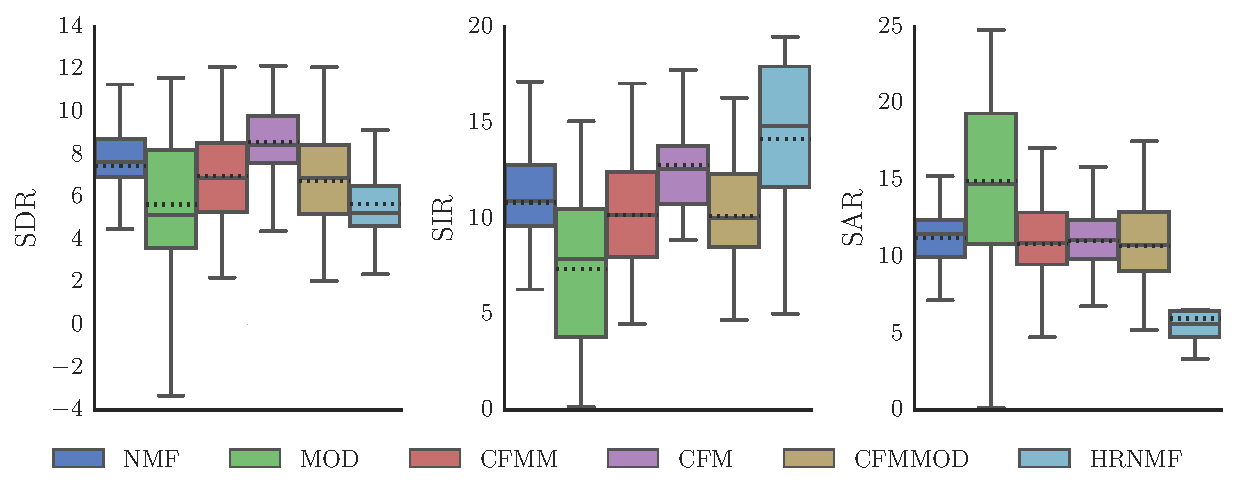
\includegraphics[width=0.8\textwidth]{Chapters/06_Separation_Unknown/figures/cfm_boxplot.pdf}
\caption{Boxplots of BSS-Eval results of the unison dataset. Solid/dotted lines represent medians/means.}
\label{fig:boxplot_overall}
\end{figure}

\begin{figure}[ht!]
\centering
		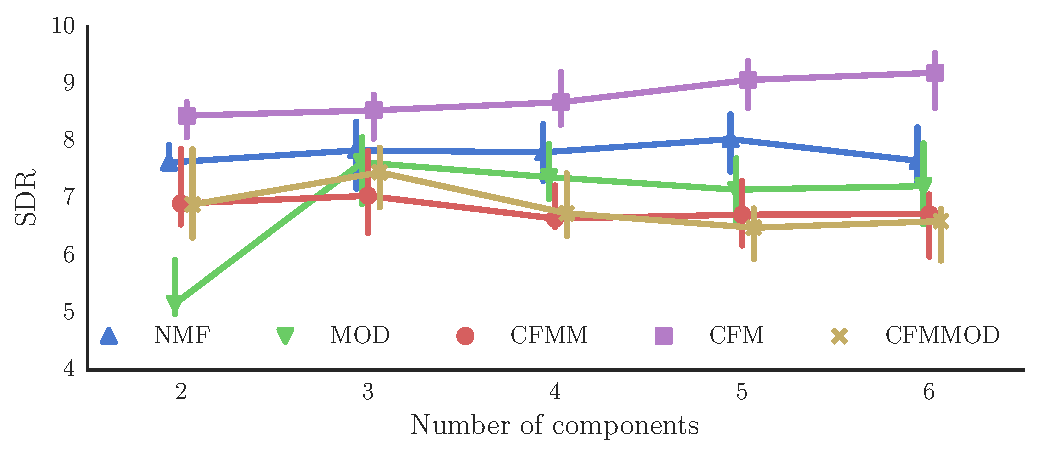
\includegraphics[width=0.8\textwidth]{Chapters/06_Separation_Unknown/figures/iterations.pdf}
\caption{Boxplots of SDR values of the unison dataset over the number of components $j$. For $j>2$ oracle clustering was applied.}
\label{fig:iterations}
\end{figure}

% TODO: move conclusion somewhere else
In this work we presented a method to exploit common modulation textures for source separation. A transformation based on a complex tensor representation computed from patches of the STFT has been introduced. We then showed how these patches are factorized by the proposed \emph{Common Fate Model}, which is derived from the idea of humans perceiving common modulation over time as one source. Our results on unisonous musical instruments indicate that this method can perform well for this scenario. The CFM model could also be successfully used in other scenarios, such as speech separation.

\section{Common Fate Model for Lead Accompaniment Separation using Deep Neural Network}

\marginpar{This section is original work being done as part of the \emph{STO1} and \emph{STO2} submission for the SiSEC 2016~\cite{sisec16}.}

In the previous section, we showed, that the common fate model is suitable to separate highly overlapped signals based on their spatial-temporal modulation texture.
In this section I show how to extend this work for the application of lead  and accompaniment separation.
This scenario is significantly more complex than the separation of single instrument notes, hence, a separation model is neede that is flexible enough to handle many of the critical edge cases which make music separation challenging.
With recent success of machine learning models, it, however, became apparent that an unsupervised model such as NTF or CFM is not flexible enough to enforce the significant amount of domain knowledge to improve performance.
% from zafar
Taking advantage of the recent availability of sufficiently large databases of isolated vocals along with their accompaniment, several researchers investigated the use of machine learning methods to directly estimate a mapping between the mixture and the sources.
There already some works based on end-to-end separation methods, processing the raw waveform~\cite{venkataramani17}.
However, most other systems today, still use classical time-frequency representations, building time-frequency masks.
\par
The common structure of a deep learning methods for lead and accompaniment separation usually corresponds to the one depicted in Figure~\ref{fig:methods_dnn}.
Most methods mainly differ in the architecture picked for the network, its input and output representation as well as in the way the network is trained.

\begin{figure}
  \centering
  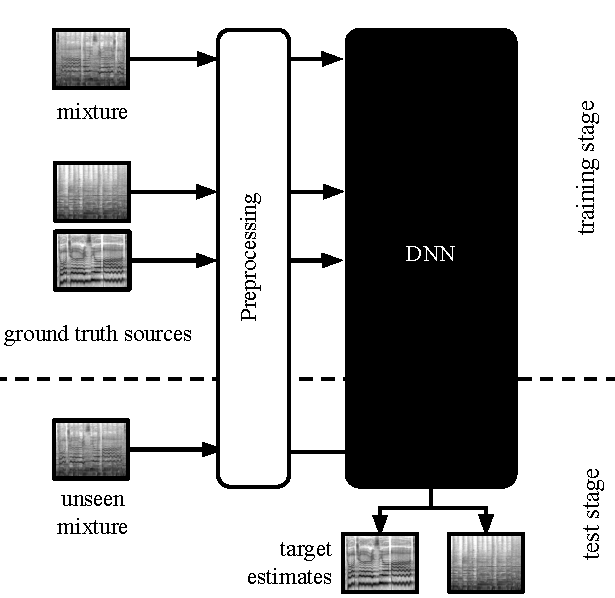
\includegraphics[width=0.6\textwidth]{Chapters/06_Separation_Unknown/figures/methods_dnn.pdf}
  % [Deep learning methods.
  %   the mixture is fed into a pre-processing step, that outputs the spectrogram. That spectrogram is input to a DNN block, which has an optional split in two parts (lead/accompaniment separate or joint). Then, we have two options for the output: either we output the mask directly, or the spectrograms to be used for building a ratio mask.
  % ]
  \caption{General architecture for methods exploiting deep learning. The network inputs the mixture and outputs either the sources spectrograms or a TF mask. Methods usually differ in their choice for a network architecture and the way it is learned using the training data.}
  \label{fig:methods_dnn}
\end{figure}

% zafar
Providing a thorough introduction to deep neural networks (DNN) is out of the scope of this thesis.
For the understanding of this section, it is sufficient to mention that DNNs consist of a cascade of several, possibly non-linear transformations of the input, which are learned during a training stage.
They were shown to effectively learn representations and mappings, provided enough data is available for estimating their parameters \cite{deng14, lecun15, goodfellow16}.
Different architectures for neural networks may be combined/cascaded together, and many architectures were proposed in the past, such as feedforward fully-connected neural networks (FNN), convolutional neural networks (CNN), or RNN and variants such as the long short-term memory (LSTM) and the gated-recurrent units (GRU).
% Training of such functions is achieved by stochastic gradient descent \cite{robbins51} and associated algorithms, such as backpropagation \cite{rumelhart862} or backpropagation through time \cite{rumelhart86} for the case of RNNs.
\par
%The first one: Huang
% zafar
Huang et al. were the first to propose deep neural networks, RNNs here \cite{hermans13,pascanu14}, for singing voice separation in \cite{huang14,huang15}. They adapted their framework from \cite{huang142} to model all sources simultaneously through masking. Input and target functions were the mixture magnitude and a joint representation of the individual sources. The objective was to estimate jointly either singing voice and accompaniment music, or speech and background noise from the corresponding mixtures.
\par
%Exploiting context: FNN with context, LSTM
Modeling the temporal structures of both the lead and the accompaniment is a considerable challenge, even when using DNN methods. As an alternative to the RNN approach proposed by Huang et al. in \cite{huang14}, Uhlich et al. proposed the usage of the simpler FNNs \cite{uhlich15} whose input consists of \textit{supervectors} of a few consecutive frames from the mixture.
This method can be described as a variant of a stacked denoising autoencoder~\cite{pvincent08}, where the noisy input is mapped to a clean output of the same dimensionality.
\par
I decided to deploy model of Uhlich~\cite{uhlich15} to evaluate the separation quality.
The aim of this work was not to exactly reproduce the results of~\cite{uhlich15}.
Instead, the objective was to evaluate one main research questions: would an DNN based model benefit from the common fate representation which is able to capture more of the modulation texture?
For the reimplementation of the model, I using the Keras~\cite{chollet15} deep learning framework to systematically assess the input-and output representation of the system.

\par
The network is a three layer FNN where each of the hidden layer has the same number of hidden nodes as the targeted output representation.
The architecture is depicted in Figure~\ref{fig:cft_dnn}.

\begin{figure}[ht!]
\centering
		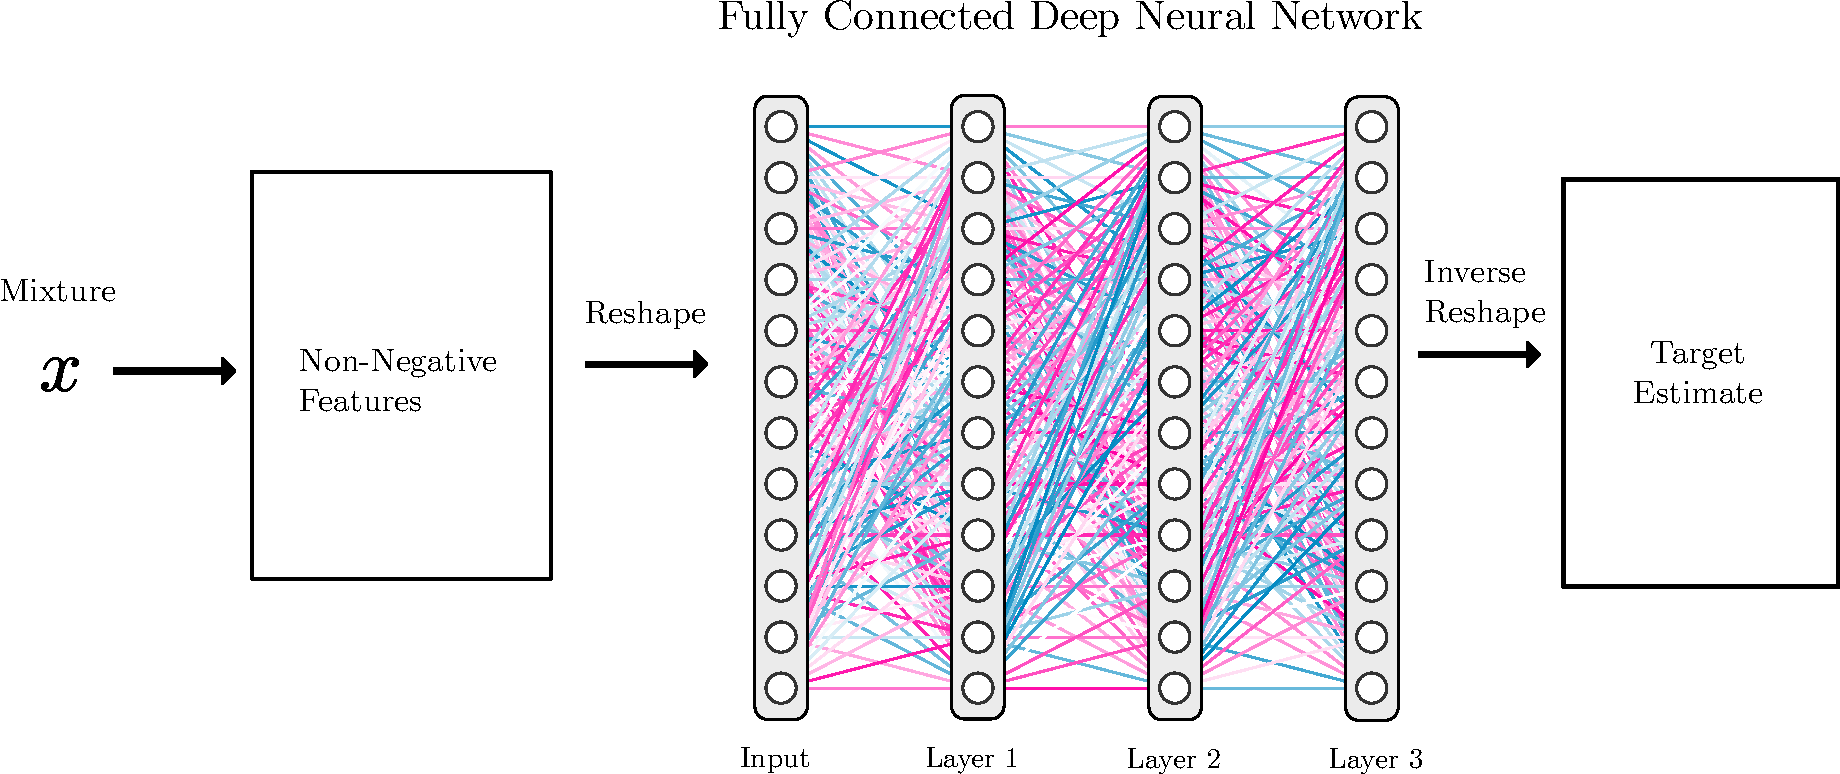
\includegraphics[width=\textwidth]{Chapters/06_Separation_Unknown/figures/uhlich_dnn.pdf}
\caption{}
\label{fig:cft_dnn}
\end{figure}

\subsection{Inputs and Outputs}

FNN networks can hardly deal with temporal structure of succeeding samples (here: frames).
Also any two-dimenionaly matrix is reshaped to a supervector to be processed by the FNN.
This makes it difficult to learn structure of neighbouring time frequency bins. However this drawback is compensated by the large number of parameters in an FNN layer.

Since the the STFT, GFT and CFT are lapped transforms different scenarios for the input and output representation of the FNN can be envisioned:

\begin{description}[style=unboxed,leftmargin=0cm]
\item[STFT-STFT]: for the \emph{input}, we compute the STFT (\(N=1024, Hop=512\) of each the audio track and select excerpts of size, \(\mathbf{X} \in \mathcal{R}^{2C + 1}_{+} \), where \(C\) is the number of preceding and succeeding frames around the central frame \(\mathbf{X}_{i+C}\). For the \emph{output}, only a single central frame \(\mathbf{Y}_{i+C}\) is selected.
I use \(C=2\), reflecting the setting in~\cite{uhlich15}. This results in an input sample size of \(\mathbf{X} \in \mathcal{R}_{+}^{5, 513}\) and  \(\mathbf{Y} \in \mathcal{R}_{+}^{1, 513}\).

\item[GFT-GFT/GFT-STFT]: instead of taking excerpts from the STFT, like in \emph{STFT-STFT}, we compute overlapping patches, as described from in Section~\ref{sub:CFT}. Each patch is of size \((5, 8)\), which means that the same number of time frames are used compared to \emph{STFT-STFT} but additionaly redundancy has been added because of the overlap between neighbouring patches.
For the \emph{output}, I chose the GFT of \(Y\).
This results in an input sample size of \(\mathbf{X} \in \mathcal{R}_{+}^{128, 5, 8}\) and  \(\mathbf{Y} \in \mathcal{R}_{+}^{128, 5, 8)}\).
Furthermore, to reduce the number of parameters, I also evaluated a setting where just the \emph{output} is the central frame of the STFT.

\item[CFT-CFT/CFT-STFT]: here, in the first step a processing as in \emph{GFT-GFT} was applied and then the 2D-DFT transform was applied (see Section~\ref{sub:CFT}).
The results in an identical shapes as in the \emph{GFT-GFT} but with added benefits of this representation can model neighbouring phase dependencies.
\end{description}

We used the DSD100 dataset~\cite{ono15} for training and test. For each sample fed into the network, we randomly select mixture tracks from the DSD100 dataset.
We then form input and output samples from these tracks, depending on the chosen input and output representation.

\subsection{Training}

To form a single sample as input for the FNN, we first compute the input representation of an audio track from the DSD100 set and then create samples by randomly sampling without replacement from these tracks.
The actual training has been done using mini-batches of size 32.
Each architecture is trained using the ADAM optimizer~\cite{kingma14} (learning rate: \(1 \cdot 10^{-3}\), \(\beta_1=0.9\), \(\beta_2=0.999\), \(\epsilon=1 \cdot 10^{-8}\))
The model was trained for a fixed number of 30 epochs and, in contrast to~\cite{uhlich15}, greedy layerwise pretraining was not applied.

\subsection{Results}

\begin{figure}[t]
\centering
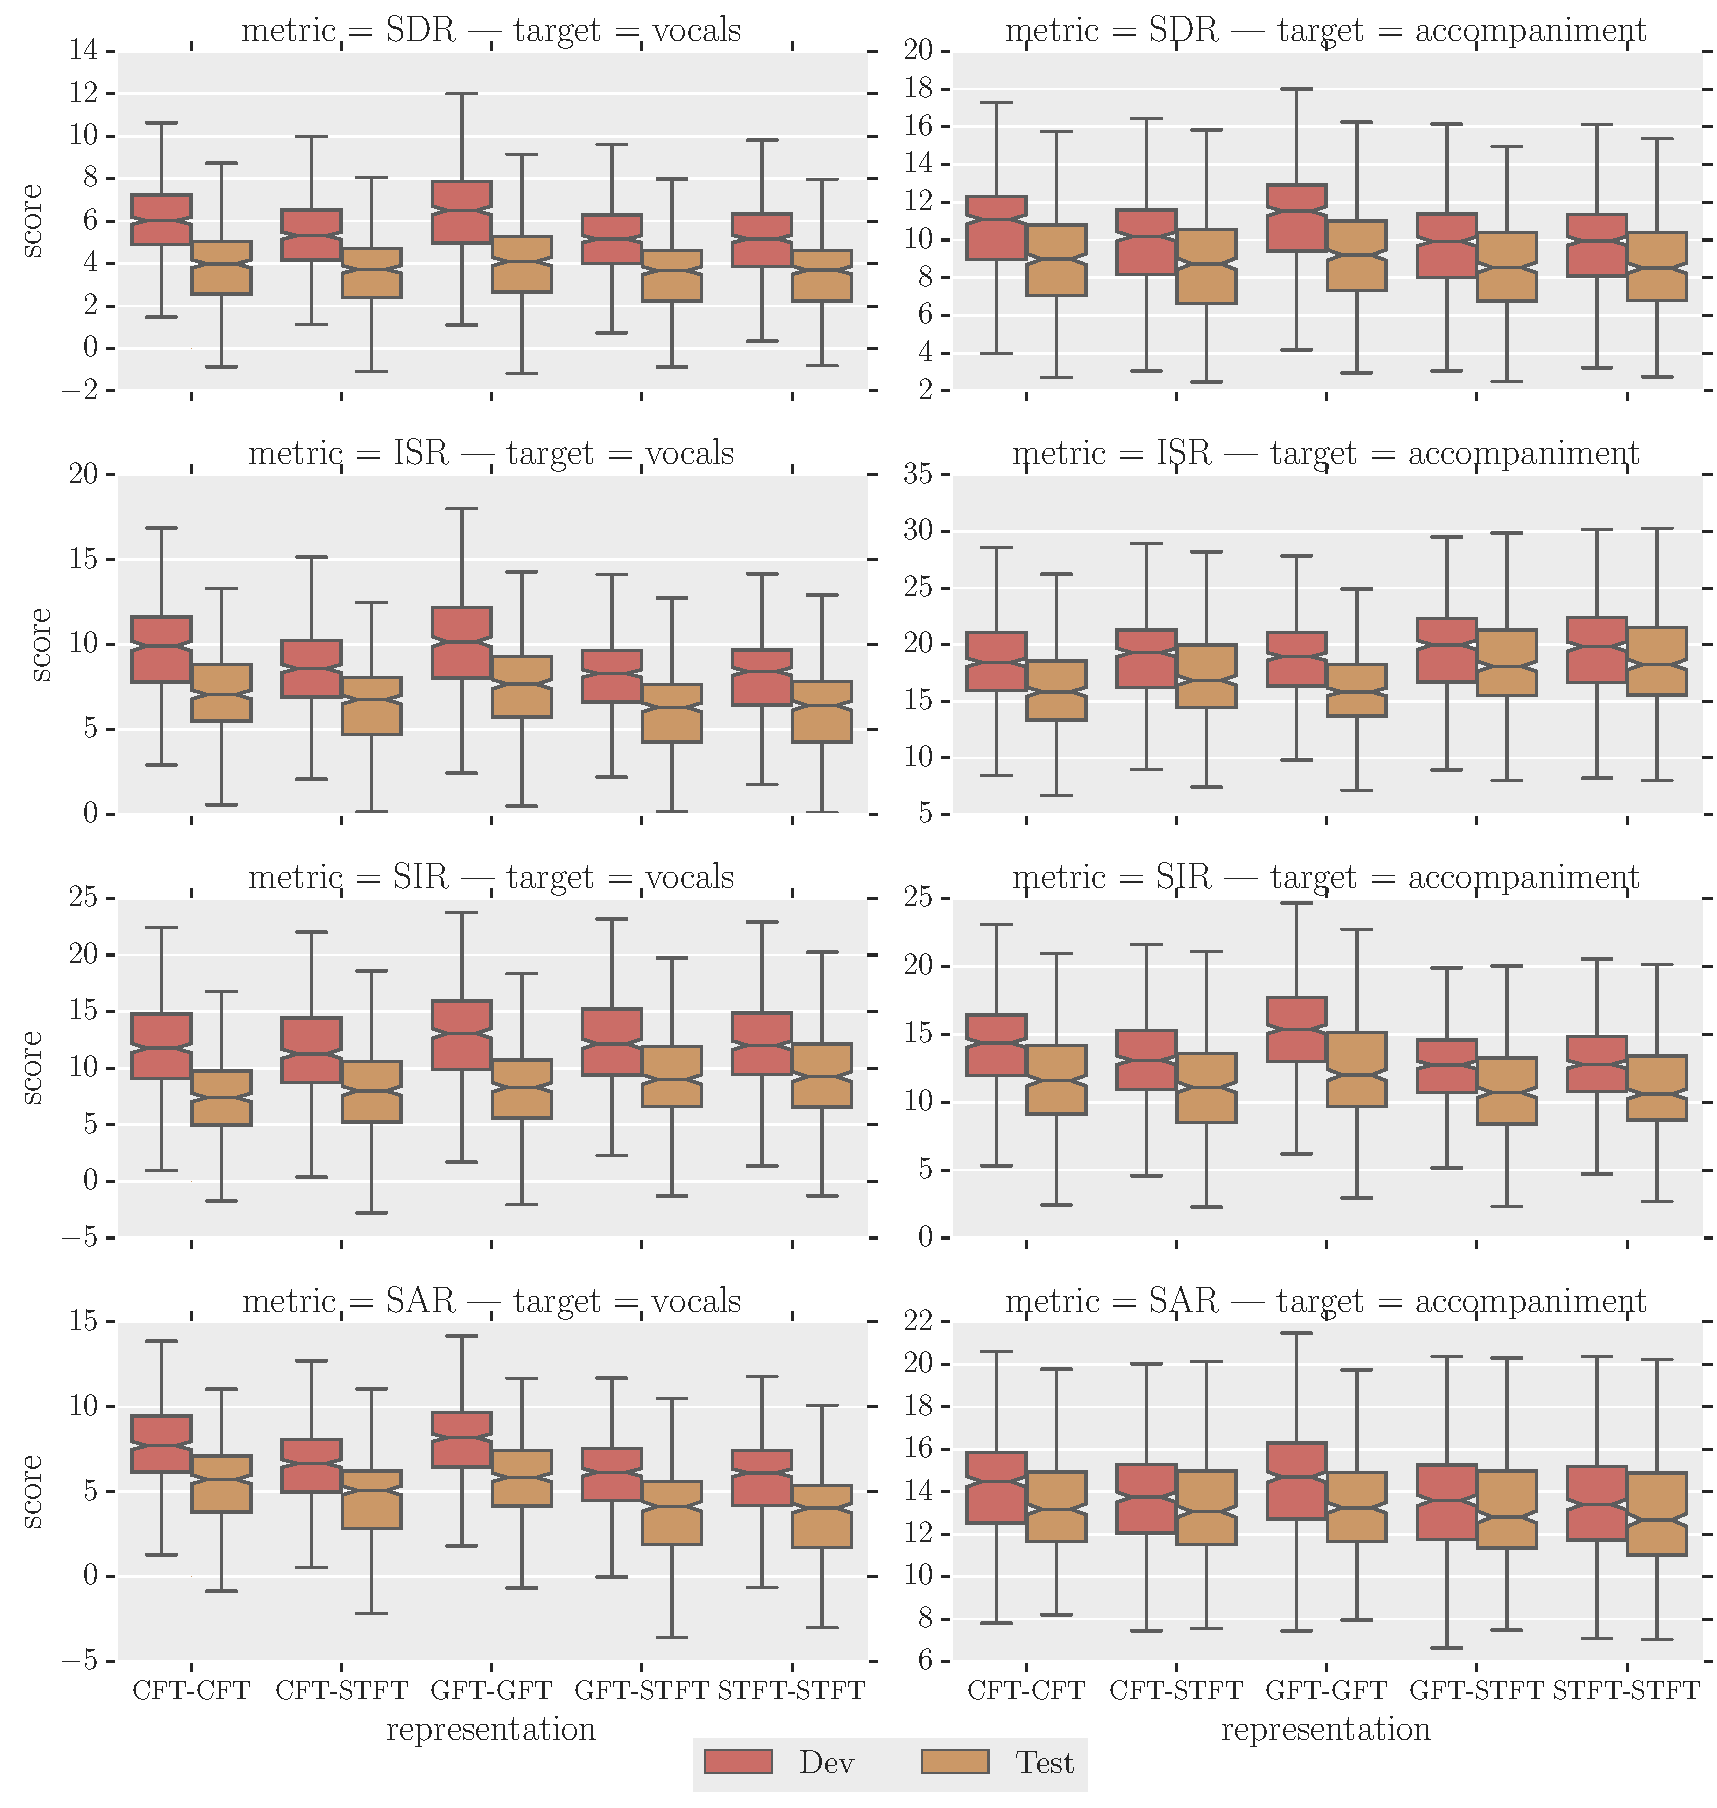
\includegraphics[width=1.0\textwidth]{Chapters/06_Separation_Unknown/figures/boxplot.pdf}
\caption{BSSEval separation results of the DSD100 dataset results for vocals and accompaniment sources. Several combinations of `input-output` were tested, as indicated by the x-axis.}
\label{fig:deep_cft_boxplots}
\end{figure}

For evaluation, the bsseval metrics of all representations for the DSD100 test set were computed.
The results are depicted in Figure~\ref{fig:deep_cft_boxplots}.
They indicate that the common fate representation is indeed improving the baseline \emph{STFT-STFT} results.
Overall, we can report a mean difference of 0.4~dB for CFT-CFT and 0.5dB for GFT-GFT, compared the \emph{STFT-STFT} representation.
However, it is worth mentioning that both, the GFT and the CFT representation lead to a signifcant increase in redundancy in the representation resulting in an increased number of trainable parameters per network layer (26219520 for CFT vs 263682 for STFT).

\subsection{Submission to SiSEC 2016}
\label{ssec:performance}

\marginpar{Parts of this subsection has been published for the SiSEC 2016~\cite{sisec16} which was coorganized by me.}

The results result have beend submitted to the 2016 SiSEC source separation challenge.
Therefore I am able to relate my work in comparison to $22$ other source separation methods, all evaluated on the same test data, as part of the task for separating professionally-produced music recordings at SiSEC 2016.
Table~\ref{tab:sisec_systems} lists the participating systems.
\begin{table*}[htbp]
	\centering
	\caption{Methods evaluated during SiSEC 2016.}
	\label{tab:sisec_systems}
	\begin{tabular}{lll@{}}
		\hline
		\textbf{Acronym} & \textbf{Ref.} & \textbf{Summary}\\
		\hline
    STO1-2 & Proposed & FNN on \textit{common fate} TF representation \\
		HUA & \cite{huang12} & RPCA standard version \\
		RAF1 & \cite{rafii13} & REPET standard version \\
		RAF2 & \cite{liutkus12} & REPET with time-varying period \\
		RAF3 & \cite{rafii12} & REPET with similarity matrix \\
		KAM1-2 & \cite{liutkus15} & KAM with different configurations \\
		CHA & \cite{chan15} & RPCA with vocal activation information \\
		JEO1-2 & \cite{jeong17} &  $l_1$-RPCA with vocal activation information \\
		DUR & \cite{durrieu11} & Source-filter NMF \\
		OZE & \cite{salaun14} & Structured NMF with learned dictionaries \\
		KON & \cite{huang15} & RNN \\
		GRA2-3 & \cite{grais16} & DNN ensemble \\
		UHL1 & \cite{uhlich15} & FNN with context \\
		NUG1-4 & \cite{nugraha16} & FNN with multichannel information \\
		UHL2-3 & \cite{uhlich17} & LSTM with multichannel information \\
		IBM & & ideal binary mask \\
	\end{tabular}
\end{table*}

%announcing the results and the webpage
The objective scores for these methods were obtained using BSS Eval and are given in Figure~\ref{fig:eval}.

\begin{figure*}[htbp]
	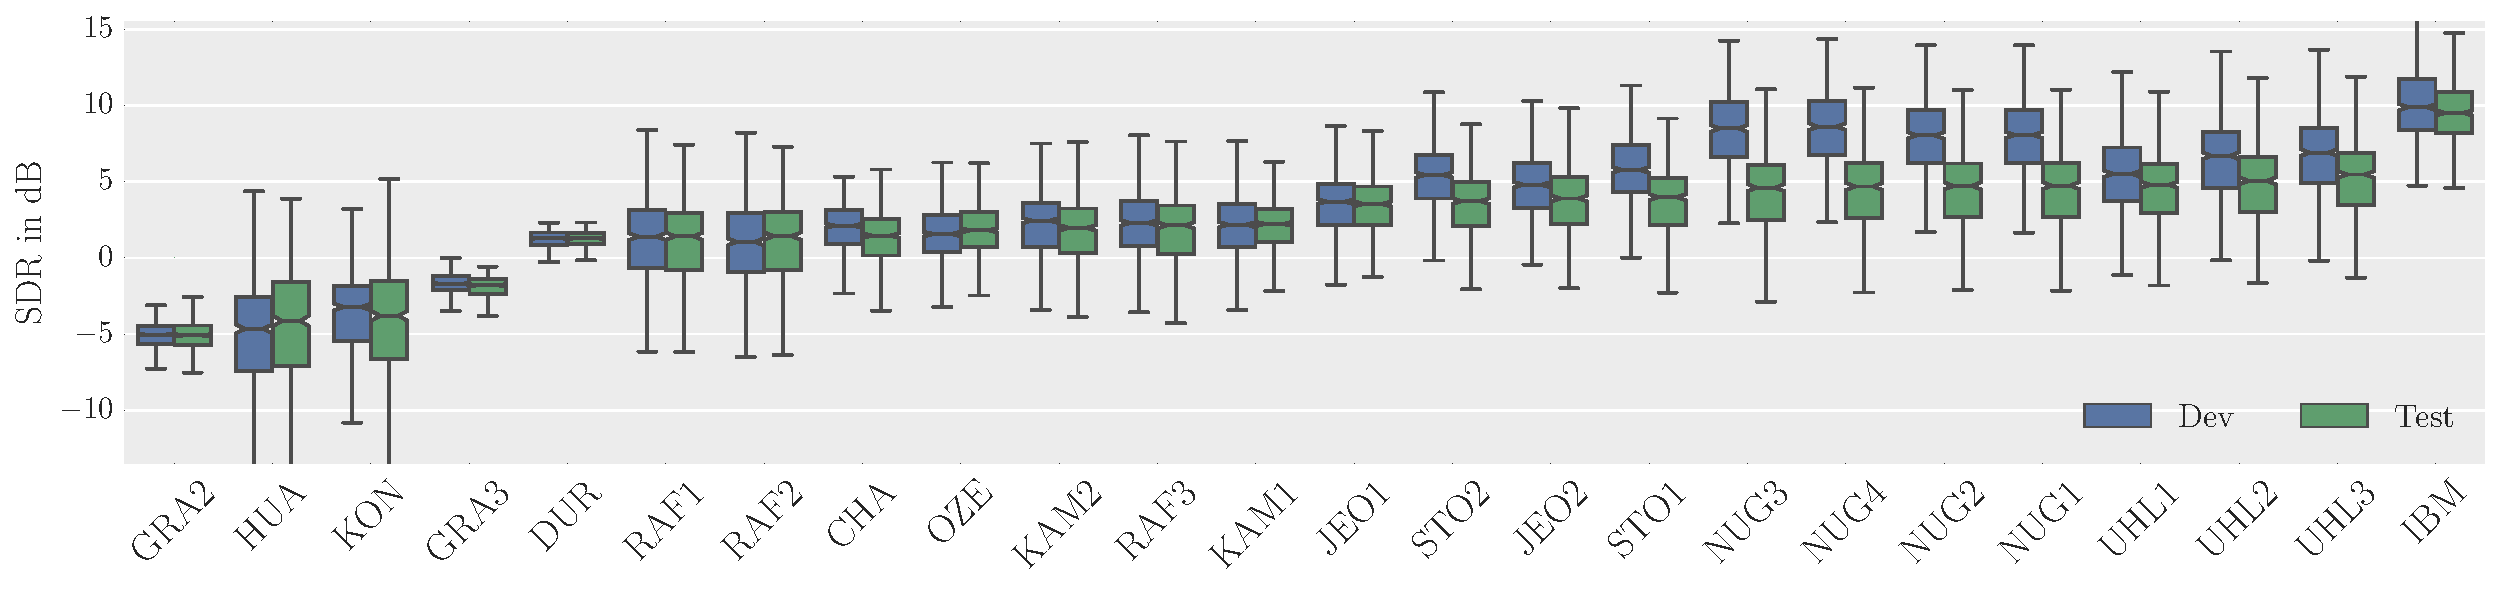
\includegraphics[width=\textwidth]{gfx/vocalsSDR.pdf}
	\caption{BSS Eval scores for the vocals and accompaniment estimates for SiSEC 2016 on the DSD100 dataset. Results are  shown for the \emph{test} set only. Scores are grouped as in Table~\ref{tab:systems} according to the section they are described in the text, indicated below each group.}
	\label{fig:eval}
\end{figure*}

%RPCA suffers from full-length recordings
As first notice in Figure~\ref{fig:eval}, the HUA method showed rather disappointing performance in this evaluation. After inspection of the results, it appears that processing full-length tracks is the issue there: at such scales, vocals also exhibit redundancy, which is captured by the low-rank model associated with the accompaniment. On the other hand, the RAF1-3 and KAM1-3 methods that exploit redundancy through repetitions, as presented in Section~\ref{ssec:methods_repet}, behave much better for full-length tracks: even if somewhat redundant, vocals are rarely as repetitive as the accompaniment. When those methods are evaluated on datasets with very short excerpts (e.g., MIR-1K), such severe practical drawbacks are not apparent.

%DUR also+non harmonic lead
Likewise, the DUR method that jointly models the vocals as harmonic and the accompaniment as redundant, as discussed in Section~\ref{ssec:methods_sourcefilter}, does show rather disappointing performance, considering that it was long the state-of-the-art in earlier SiSECs \cite{vincent12}. After inspection, we may propose two reasons for this performance drop. First, using full-length excerpts also clearly revealed a shortcoming of the approach: it poorly handles silences in the lead, which were rare in the short-length excerpts tested so far. Second, using a much larger evaluation set revealed that vocals are not necessarily well modeled by a harmonic source-filter model; breathy or saturated voices appear to greatly challenge such a model.

%RPCA informed by lead presence behaves well
While processing full-length tracks comes as a challenge, it can also be an opportunity. It is indeed worth noticing that whenever RPCA is helped through vocal activity detection, its performance is significantly boosted, as highlighted by the relatively good results obtained by CHAN and JEO.

%OZE could benefit from the new learning data
As discussed in Section~\ref{sec:datadriven-approaches}, the availability of learning data made it possible to build data-driven approaches, like the NMF-based OZE method which is available through the Flexible Audio Source Separation Toolbox (FASST) \cite{salaun14,ozerov12}. Although it was long state-of-the-art, it has been strongly outperformed recently by other data-driven approaches, namely DNNs. One first reason clearly appears as the superior expressive power of DNNs over NMF, but one second reason could very simply be that OZE should be trained anew with the same large amount of data.

%DNN are definitely performing awesomely
As mentioned above, a striking fact we see in Figure~\ref{fig:eval} is that the overall performance of data-driven DNN methods is the highest. This shows that exploiting learning data does help separation greatly compared to only relying on \textit{a priori} assumptions such as the harmonicity or redundancy. Additionally, dynamic models such as CNN or LSTM appear more adapted to music than FNN. These good performances in audio source separation go in line with the recent success of DNNs in fields as varied as computer vision, speech recognition, and natural language processing \cite{lecun15}.

%but it's clear that they benefit from smart ideas
However, the picture may be seen to be more subtle than simply black-box DNN systems beating all other approaches. For instance, exploiting multichannel probabilistic models, as discussed in Section~\ref{sec:multichannel}, leads to the NUG and UHL2-3 methods, that significantly outperform the DNN methods ignoring stereo information. In the same vein, we expect other specific assumptions and musicological ideas to be exploited for further improving the quality of the separation.

%weakness of metrics
One particular feature of this evaluation is that it also shows obvious weaknesses in the objective metrics. For instance, the GRA method behaves significantly worse than any other methods. However, when listening to the separated signals, this does not seem deserved. All in all, designing new and convenient metrics that better match perception and that are specifically built for music on large datasets clearly appears as a desirable milestone.

%IBM much better: room for improvement
In any case, the performance achieved by a totally informed filtering method such as IBM is significantly higher than that of any submitted method in this evaluation. This means that lead and accompaniment separation has room for much improvement, and that the topic is bound to witness many breakthroughs still. This is even more true considering that IBM is not the best upper bound for separation performance: other filtering methods such as \textit{ideal ratio mask}~\cite{liutkus15c} or multichannel Wiener filter~\cite{duong10} may be considered as references.
\par
Relating our results of STO1 and STO2 to the other methods, we observe that our results are comparable to the state-of-the-art performance of UHL and NUG.
Also the difference between test and validation dataset indicate, that our CFT has better generalization than NUG.

For more details about the results and for listening to the estimates, we refer the reader to the dedicated interactive website\footnote{\url{http://www.sisec17.audiolabs-erlangen.de}}.

Modern JavaScript technologies like the Web Audio API make it possible to interactively assess source separation results in the browser.
For the first time, interested researchers are able to listen to over 10000 stimuli from all particiapting systems.
For track, we provide the separation results as well as the objective BSSeval scores.
Figure~\ref{fig:sisec_website} depicts a screenshot of the website.
The objective scores are depicted as interactive matrix where users are able to sort the results for each track an each system interactactively by the the source of interest.
Clicking on one ... an interactive player is opened that allows.
TODO


\begin{figure}[t]
\centering
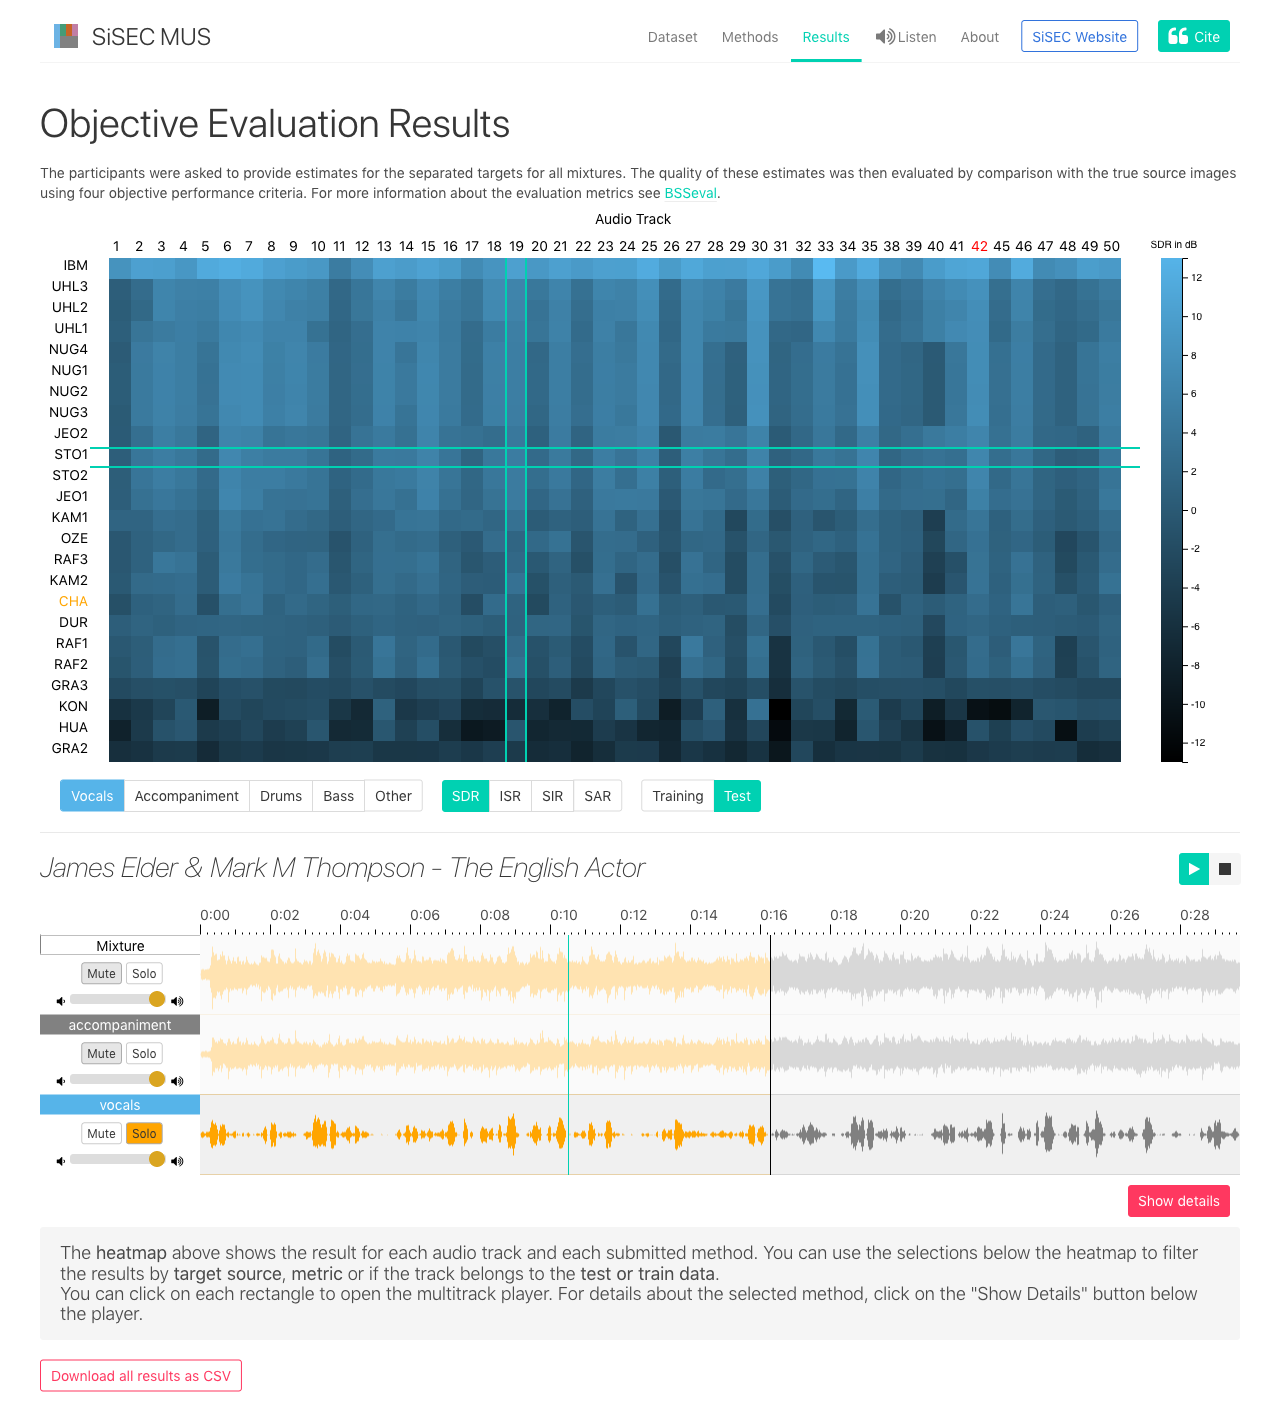
\includegraphics[width=0.9\textwidth]{Chapters/06_Separation_Unknown/figures/sisec_website.png}
\caption{Screenshot of the SiSEC 2016 Website~\url{http://sisec17.audiolabs-erlangen.de}}
\label{fig:sisec_website}

\end{figure}

\section{Chapter Summary and Discussion}

\begin{itemize}
  \item DNNs: Super-Frames are computationaly too complex and a the same time not flexible enough regarding processing of variable length input. This can be solved by recurrent models. 
  % TODO add reference to show equivalence between NMF/NTF and DNNs
  \item I evaluated the common transform in the context of deep neural network based separation.
  Todays phase aware DNNs (cite complex dnn, phasenet), are a line of research.
  \item 
  \item DNNs: Modern Architechtures, like CNNs and DNNs are more powerful but often do not significantly improve the results: SiSEC 2018. This is why domain knowledge can still be applied.
\end{itemize}
